\section{Specifica Front-End}
	\subsection{SWEDesigner::Client}
		\subsubsection{Informazioni generali}
			\begin{itemize}
          		\item \textbf{Descrizione:}\\
          		Questo package racchiude tutta la componente di Front-end scritta in TypeScript.\\
          		Gli attributi e i metodi di alcune classi saranno definiti a partire dalla prossima versione.
          		\item \textbf{Padre:} SWEDesigner
          		\item \textbf{Package contenuti:}\\
          		\begin{itemize}
          			\item Components\\
          			Questo package contiene tutti i components dell’applicazione
          			\item Services\\
          			Questo package contiene i servizi per le operazioni di iterazione tra i components e
il server
          		\end{itemize}
          	\end{itemize}
          	
		\subsubsection{Classi}
		
			\paragraph{SWEDesigner::AuthenticationGuard}
				\begin{figure}[h!]
	\centering
	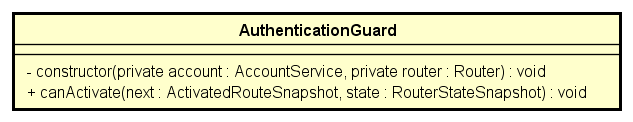
\includegraphics[scale=0.8]{res/sections/SpecificaFrontEnd/Services/Disegnetti/authenticationguard.png}
	\caption{Diagramma della classe AuthenticationGuard}
\end{figure}

\begin{itemize}
	\item \textbf{Descrizione:}\\
	Servizio che permette la verifica dell'utente durante l'autenticazione.
	
	\item \textbf{Utilizzo:}\\
	Utilizzato per verificare l'autenticazione dell'utente
	\item \textbf{Metodi:}
		\begin{itemize}
			\item \emph{-constructor( private account: AccountService, private router: Router)}\\
    		Costruttore della classe\\
    		\textbf{Parametri:}
    		\begin{itemize}
    			\item \emph{account: AccountService}\\
    			Crea un istanziazione di AccountService
    			\item \emph{router: Router}\\
    			Crea un istanziazione di Router
    		\end{itemize}
    		\item \emph{+canActivate(next: ActivatedRouteSnapshot, state: RouterStateSnapshot)}\\
    		\\
    		\textbf{Parametri:}
    		\begin{itemize}
    			\item \emph{next: ActivatedRouteSnapshot}\\
    			Un metodo dell'interfaccia
    			\item \emph{state: RouterStateSnapshot}\\
    			Un booleano dell'interfaccia
    		\end{itemize}
		\end{itemize}
\end{itemize}
				
			\paragraph{SWEDesigner::Global}
				%%%%%%%%%%%%%%
%  COSTANTI  %
%%%%%%%%%%%%%%

% In questa prima parte vanno definite le 'costanti' utilizzate da due o pi� documenti.

% Meglio non mettere gli \emph dentro le costanti, in certi casi creano problemi
\newcommand{\GroupName}{SWEet BIT}
\newcommand{\GroupEmail}{sweet.bit.group@gmail.com}
\newcommand{\ProjectName}{SWEDesigner}
\newcommand{\ProjectVersion}{v1.0.0}

\newcommand{\Proponente}{Zucchetti Spa}
\newcommand{\Committente}{Prof. Tullio Vardanega \\ Prof. Riccardo Cardin}
\newcommand{\Responsabile}{Da Decidere}

% La versione dei documenti deve essere definita qui in global, perch� serve anche agli altri documenti
\newcommand{\VersioneG}{1.0.0}
\newcommand{\VersionePQ}{1.2.0}
\newcommand{\VersioneNP}{1.2.0}
\newcommand{\VersionePP}{1.2.0}
\newcommand{\VersioneAR}{1.2.0}
\newcommand{\VersioneSF}{1.2.0}
\newcommand{\VersioneST}{1.0.0}
\newcommand{\VersioneMA}{1.0.0}
\newcommand{\VersioneMS}{1.0.0}
\newcommand{\VersioneMU}{1.0.0}
\newcommand{\VersioneDP}{1.0.0}
\newcommand{\VersioneVE}{1.3.0}
% Il verbale non ha versionamento.

% Quando serve riferirsi a ``Nome del Documento + ultima versione x.y.z'' usiamo queste costanti:
\newcommand{\Glossario}{\emph{Glossario v\VersioneG{}}}
\newcommand{\PianoDiQualifica}{\emph{Piano di Qualifica v\VersionePQ{}}}
\newcommand{\NormeDiProgetto}{\emph{Norme di Progetto v\VersioneNP{}}}
\newcommand{\PianoDiProgetto}{\emph{Piano di Progetto v\VersionePP{}}}
\newcommand{\StudioDiFattibilita}{\emph{Studio di Fattibilit� v\VersioneSF{}}}
\newcommand{\AnalisiDeiRequisiti}{\emph{Analisi dei Requisiti v\VersioneAR{}}}
\newcommand{\SpecificaTecnica}{\emph{Specifica Tecnica v\VersioneST{}}}
\newcommand{\ManualeAdmin}{\emph{Manuale Admin v\VersioneMA{}}}
\newcommand{\ManualeSviluppatore}{\emph{Manuale Sviluppatore v\VersioneMS{}}}
\newcommand{\ManualeUtente}{\emph{Manuale Utente v\VersioneMU{}}}
\newcommand{\DefinizioneDiProdotto}{\emph{Definizione di Prodotto v\VersioneDP{}}}

\newcommand{\ScopoDelProdotto}{
	Lo scopo del progetto � la realizzazione del progetto \glossaryItem{SWEDesigner}.}

%%%%%%%%%%%%%%
%  FUNZIONI  %
%%%%%%%%%%%%%%

% In questa seconda parte vanno definite le 'funzioni' utilizzate da due o pi� documenti.

% Serve a dare la giusta formattazione alle parole presenti nel glossario
% il nome del comando \glossary � gi� usato da LaTeX
\newcommand{\glossaryItem}[1]{\textit{#1\ped{\ped{G}}}}

% Serve a dare la giusta formattazione per indicare il tipo di verbale in cui e' stata presa una decisione
% Uso: \verbalRI{data}{punto}
% RI = Riunione Interna
\newcommand{\verbalRI}[2]{\textit{RI-#1-#2}}
% RE = Riunione Esterna
\newcommand{\verbalRE}[2]{\textit{RE-#1-#2}}

% Serve a dare la giusta formattazione al codice inline
\newcommand{\code}[1]{\flextt{\texttt{#1}}}

% Serve a dare la giusta formattazione a tutte le path presenti nei documenti
\newcommand{\file}[1]{\flextt{\texttt{#1}}}

% Permette di andare a capo all'interno di una cella in una tabella
\newcommand{\multiLineCell}[2][c]{\begin{tabular}[#1]{@{}l@{}}#2\end{tabular}}

% Genera automaticamente la pagina di copertina
\newcommand{\makeFrontPage}{
  % Declare new goemetry for the title page only.
  \newgeometry{top=3.5cm}
  
  \begin{titlepage}
  \begin{center}

  \begin{center}
  
\includegraphics[width=10cm]{../../common/logo.jpg}
  \end{center}
  
  \vspace{1cm}

  \begin{Huge}
  \textbf{\DocTitle{}}
  \end{Huge}
  
  \textbf{\emph{Gruppo \GroupName{} \, \texttwelveudash{} \, Progetto \ProjectName{}}}
  
  \vspace{11pt}

  \bgroup
  \def\arraystretch{1.3}
  \begin{tabular}{ r|l }
    \multicolumn{2}{c}{\textbf{Informazioni sul documento}} \\
    \hline
		% differenzia a seconda che \DocVersion{} stampi testo o no
		\setbox0=\hbox{\DocVersion{}\unskip}\ifdim\wd0=0pt
			% nulla (non ho trovato come togliere l'a capo)
			\\
		\else
			\textbf{Versione} & \DocVersion{} \\
		\fi
    \textbf{Redazione} & \multiLineCell[t]{\DocRedazione{}} \\
    \textbf{Verifica} & \multiLineCell[t]{\DocVerifica{}} \\
    \textbf{Approvazione} & \multiLineCell[t]{\DocApprovazione{}} \\
    \textbf{Uso} & \DocUso{} \\
    \textbf{Distribuzione} & \multiLineCell[t]{\DocDistribuzione{}} \\
  \end{tabular}
  \egroup

  \vspace{22pt}

  \textbf{Descrizione} \\
  \DocDescription{}

  \end{center}
  \end{titlepage}
  
  % Ends the declared geometry for the titlepage
  \restoregeometry
}
          	
	\subsection{SWEDesigner::Client::Components}
		\subsubsection{Informazioni generali}
			\begin{itemize}
          		\item \textbf{Descrizione:}\\
          		Questo package contiene tutti i components dell’applicazione.
          		\item \textbf{Padre:} SWEDesigner::Client
          		\item \textbf{Package contenuti:}\\
          		\begin{itemize}
          			\item Editor-container\\
          			Il package contiene tutti i components riguardanti l'editor e la gestione dell'utente
          		\end{itemize}
          	\end{itemize}
          	
		\subsubsection{Classi}
		
			\paragraph{SWEDesigner::Client::Components::RegistrationComponent}
				\begin{itemize}
    \item \textbf{Descrizione:}\\
    È il componente che descrive la pagina di registrazione dell’applicazione, mette a disposizione dell’utente un form dove iserire le informazioni necessarie alla creazione di un nuovo account utente. Gestisce le operazioni e la logica applicativa per la registrazione.
    \item \textbf{Utilizzo:}\\
    Questo componente viene istanziato dinamicamente dal servizio Router del framework Angular quando viene richiesta la pagina di registrazione.
	\item \textbf{Metodi:}
    \begin{itemize}
    	\item \emph{-constructor(private router: Router, private accountService: AccountService)}\\
    	Crea un istanziazione di RegistrationComponent
    	\item \textbf{Parametri:}
    		\begin{itemize}
    			\item \emph{-router: Router}
    			Necessario per l'importaziine del Router
    			\item \emph{-accountService: AccountService}
    			Necessario per l'importazione di AccountService
    		\end{itemize}
    	\item \emph{-tryRegistration(e: any)}\\
    	Tenta di registrare un utente
    	\item \textbf{Parametri:}
    		\begin{itemize}
    			\item \emph{+e: any}\\
    			Contiente i dati dell'utente da registrare
    		\end{itemize}
    \end{itemize}
\end{itemize}
				
			\paragraph{SWEDesigner::Client::Components::LoginComponent}
				\begin{figure}[h!]
	\centering
	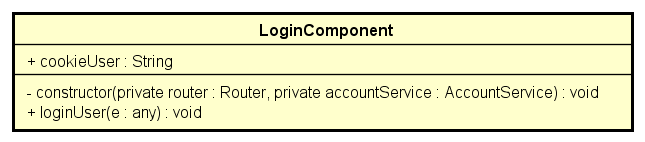
\includegraphics[scale=0.8]{res/sections/SpecificaFrontEnd/Components/Disegnetti/login.png}
	\caption{Diagramma della classe LoginComponent}
\end{figure}

\begin{itemize}
	\item \textbf{Descrizione:}\\
	È il componente che descrive la pagina di login dell’applicazione, mette a disposizione dell’utente un form dove inserire username e password. Gestisce le operazioni e la logica applicativa per il login.
	\item \textbf{Utilizzo:}\\
	Questo componente viene istanziato dinamicamente dal servizio Router del framework Angular quando viene richiesta la pagina di login.
	\item \textbf{Attributi:}
		\begin{itemize}
			\item \emph{+cookieUser: String}\\
			Riceve l'username dai cookie di sessione
		\end{itemize}
	\item \textbf{Metodi:}
		\begin{itemize}
			\item \emph{-constructor(private router: Router, private accountService: AccountService)}\\
    		Crea un istanziazione di RegistrationComponent\\
    		\textbf{Parametri:}
    		\begin{itemize}
    			\item \emph{-router: Router}
    			Necessario per l'importaziine del Router
    			\item \emph{-accountService: AccountService}
    			Necessario per l'importazione di AccountService
    		\end{itemize}
    		\item \emph{+loginUser(e: any)}\\
    		Effettua l'autenticazione dell'utente\\
    		\textbf{Parametri:}
    		\begin{itemize}
    			\item \emph{+e: any}
    			Contiente i dati dell'utente da autenticare
    		\end{itemize}
		\end{itemize}
\end{itemize}
				
			\paragraph{SWEDesigner::Client::Components::Forgot-pswComponent}
				\begin{itemize}
	\item \textbf{Descrizione:}\\
	È il componente che descrive la pagina per il recupero della password dell'applicazione, mette a disposizione un form in cui inserire l'indirizzo email. Gestisce le operazioni e la logica applicativa relativa al recupero della password.
	\item \textbf{Utilizzo:}\\
	Questo componente viene istanziato dinamicamente dal servizio Router del framework Angular quando viene richiesta la pagina di password dimenticata.
	\item \textbf{Metodi:}
		\begin{itemize}
			\item \emph{-constructor(private accountService: AccountService)}\\
    	Crea un istanziazione di Forgot-pswComponent
    	\item \textbf{Parametri:}
    		\begin{itemize}
    			\item \emph{-accountService: AccountService}
    			Necessario per l'importazione di AccountService
    		\end{itemize}
    		\item \emph{+tryGetNewPassword(e: any)}\\
    		Invia all'utente la password per email
    	\item \textbf{Parametri:}
    		\begin{itemize}
    			\item \emph{+e: any}
    			Contiente i dati dell'utente che ha richiesto il recupero password
    		\end{itemize}
		\end{itemize}
\end{itemize}
				
	\subsection{SWEDesigner::Client::Components::Editor-container}
		\subsubsection{Informazioni generali}
			\begin{itemize}
          		\item \textbf{Descrizione:}\\
          		Questo package contiene tutti i components riguardanti l'editor e la gestione dell'utente.
          		\item \textbf{Padre:} SWEDesigner::Client::Components
          		\item \textbf{Package contenuti:}\\
          		\begin{itemize}
          			\item Menu\\
          			Il package contiene tutti i components riguardanti la gestione delle funzionalità offerte dal menu
          			\item Editor\\
          			Il package contiene tutti i components riguardanti l'editor e la gestione dell'utente
          		\end{itemize}
          	\end{itemize}
          	
		\subsubsection{Classi}
		
			\paragraph{SWEDesigner::Client::Components::Editor-container::Editor-containerComponent}
				\begin{itemize}
	\item \textbf{Descrizione:}\\
	È il componente che contiene il componente del menù e quello dell'editor.
	\item \textbf{Utilizzo:}\\

	\item \textbf{Attributi:}
		\begin{itemize}
			\item \emph{-selectedGraph: any}\\
			Punta al graph corrente.
		\end{itemize}
	\item \textbf{Metodi:}
		\begin{itemize}
			\item \emph{-constructor(private menuService: MenuService,
    private accountService: AccountService)}\\
    		Costruttore della classe\\
    		\textbf{Parametri:}
    		\begin{itemize}
    			\item \emph{menuService: MenuService}\\
    			Crea un istanziazione di MenuService  			
    			\item \emph{accountService: AccountService}\\
    			Crea un istanaziazione di AccountService
    		\end{itemize}
\end{itemize}
				
			\paragraph{SWEDesigner::Client::Components::Editor-container::Activity-frameComponent}
				\input{res/sections/SpecificaFrontEnd/Components/activity-frame.tex}
				
	\subsection{SWEDesigner::Client::Components::Editor-container::Menu}
		\subsubsection{Informazioni generali}
			\begin{itemize}
          		\item \textbf{Descrizione:}\\
          		Questo package contiene tutti i components riguardanti la gestione delle funzionalità offerte dal menu.
          		\item \textbf{Padre:} SWEDesigner::Client::Components::Editor-container
          	\end{itemize}
          	
          \subsubsection{Classi}
          
          	\paragraph{SWEDesigner::Client::Components::Editor-container::Menu::MenuComponent}
				\begin{itemize}
	\item \textbf{Descrizione:}\\
	
	\item \textbf{Utilizzo:}\\
	
	\item \textbf{Attributi:}
		\begin{itemize}
			\item \emph{-selectedGraphService: Subject<any>}\\
			
			\item \emph{-importData: any}\\
			
		\end{itemize}
	\item \textbf{Metodi:}
		\begin{itemize}
			\item \emph{+zoomIn()}\\
    		Esegue lo zoom in avanti
    		\item \emph{+zoomOut()}\\
    		Esegue lo zoom all'indietro
    		\item \emph{+copyElement()}\\
    		Copia l'elemento selezionato
    		\item \emph{+pasteElement()}\\
    		Incolla l'elemento copiato/tagliato
    		\item \emph{+cutElement()}\\
    		Taglia l'elemento selezionato
    		\item \emph{+undo()}\\
    		Annulla l'ultima operazione
    		\item \emph{+redo()}\\
    		Ripristina l'azione annullata
    		\item \emph{+elimina()}\\
    		Elimina l'elemento selezionato
    		\item \emph{+saveData(proj: JSON, cb: Function)}\\
    		Richiede al server dei dati del progetto corrente memorizzati nel database\\
    		\textbf{Parametri:}
    		\begin{itemize}
    			\item \emph{proj: JSON}\\
    			Progetto corrente
    			\item \emph{cb: Function}\\
    			
    		\end{itemize}
    		\item \emph{+updateData(proj: JSON, cb: Function)}\\
    		Aggiorna i dati del progetto corrente nel database\\
    		\textbf{Parametri:}
    		\begin{itemize}
    			\item \emph{proj: JSON}\\
    			Progetto corrente
    			\item \emph{cb: Function}\\
    			
    		\end{itemize}
    		\item \emph{+updateName(usr: string, oldName: string, newName: string, cb: Function)}\\
    		Aggiorna il nome del progetto corrente\\
    		\textbf{Parametri:}
    		\begin{itemize}
    			\item \emph{usr: string}\\
    			Nome utente
    			\item \emph{oldName: string}\\
    			Vecchio nome del progetto
    			\item \emph{newName: string}\\
    			Nuovo nome del progetto
    			\item \emph{cb: Function}\\
    			
    		\end{itemize}
    		\item \emph{+encrypt(proj: JSON)}\\
    		Richiede al server la funzione di criptazione\\
    		\textbf{Parametri:}
    		\begin{itemize}
    			\item \emph{proj: JSON}\\
    			Progetto da criptare
    		\end{itemize}
    		\item \emph{+readFile(file: any, onloadCallBack: any)}\\
    		Legge un file esterno\\
    		\textbf{Parametri:}
    		\begin{itemize}
    			\item \emph{file: any}\\
    			File da caricare
    			\item \emph{onloadCallBack: any}\\
    			
    		\end{itemize}
    		\item \emph{+import(event: any)}\\
    		Importa un file esterno\\
    		\textbf{Parametri:}
    		\begin{itemize}
    			\item \emph{event: any}\\
    			File da importare
    		\end{itemize}
    		\item \emph{+getImportData()}\\
    		
    		\item \emph{+donwload()}\\
    		Richiede al server la funzione di parsing e download
    		\item \emph{+code()}\\
    		Richiama la funziona di download
		\end{itemize}
\end{itemize}
				
          	\paragraph{SWEDesigner::Client::Components::Editor-container::Menu::FileComponent}
				\begin{itemize}
	\item \textbf{Descrizione:}\\
	È il componente che descrive la voce \textit{File} del menu dell'editor.
	\item \textbf{Utilizzo:}\\
	
	\item \textbf{Attributi:}
		\begin{itemize}
			\item \emph{nome_progetto: string}\\
			Contiene il nome del progetto corrente
		\end{itemize}
	\item \textbf{Metodi:}
		\begin{itemize}
			\item \emph{-constructor(private menuService: MenuService,
    private mainEditorService: MainEditorService,
    private accountService: AccountService)}\\
    		\\
    		\textbf{Parametri:}
    		\begin{itemize}
    			\item \emph{menuService: MenuService}\\
    			
    			\item \emph{mainEditorService: MainEditorService}\\
    			
    			\item \emph{accountService: AccountService}\\
    			
    		\end{itemize}
    		\item \emph{-save(projName: string)}\\
    		Memorizza un progetto nel database\\
    		\textbf{Parametri:}
    		\begin{itemize}
    			\item \emph{projName: string}\\
    			Nome del progetto da memorizzare
    		\end{itemize}
    		\item \emph{-updateProj()}\\
    		Aggiorna un progetto esistente
    		\item \emph{-export()}\\
    		Esporta il progetto corrente
    		\item \emph{-generate()}\\
    		Genera il codice Java
    		\item \emph{-import(event)}\\
    		Importa un progetto esistente\\
    		\textbf{Parametri:}
    		\begin{itemize}
    			\item \emph{event: any}\\
    			Progetto da importare
    		\end{itemize}
		\end{itemize}
\end{itemize}
				
          	\paragraph{SWEDesigner::Client::Components::Editor-container::Menu::ModificaComponent}
				\begin{figure}[h!]
	\centering
	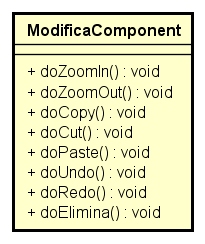
\includegraphics[scale=0.8]{res/sections/SpecificaFrontEnd/Components/Disegnetti/modifica.png}
	\caption{Diagramma della classe ModificaComponent}
\end{figure}

\begin{itemize}
	\item \textbf{Descrizione:}\\
	È il componente che descrive la voce \textit{Modifica} del menu dell'editor.
	\item \textbf{Utilizzo:}\\
	
	\item \textbf{Metodi:}
		\begin{itemize}
			\item \emph{+doZoomIn()}\\
    		Esegue lo zoon in avanti
    		\item \emph{+doZoomOut()}\\
    		Esegue lo zoom in indietro
    		\item \emph{+doCopy()}\\
    		Esegue il comando copia del menu
    		\item \emph{+doCut()}\\
    		Esegue il comando taglia del menu
    		\item \emph{+doPaste()}\\
    		Esegue il comando incolla del menu
    		\item \emph{+doUndo()}\\
    		Annulla l'ultima azione compiuta
    		\item \emph{+doRedo()}\\
    		Ripristina l'ultima azione annullata
    		\item \emph{+doElimina()}\\
    		Elimina l'elemento selezionato nell'editor	    		
		\end{itemize}
\end{itemize}
				
          	\paragraph{SWEDesigner::Client::Components::Editor-container::Menu::ProfiloComponent}
				\begin{figure}[h!]
	\centering
	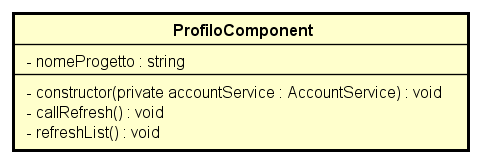
\includegraphics[scale=0.8]{res/sections/SpecificaFrontEnd/Components/Disegnetti/profilo.png}
	\caption{Diagramma della classe ProfiloComponent}
\end{figure}

\begin{itemize}
	\item \textbf{Descrizione:}\\
	È il componente che descrive la voce \textit{Profilo} del menu dell'editor.
	\item \textbf{Utilizzo:}\\
	
	\item \textbf{Attributi:}
		\begin{itemize}
			\item \emph{-nomeProgetto: string}\\
			Contiene il nome del progetto corrente
		\end{itemize}
	\item \textbf{Metodi:}
		\begin{itemize}
			\item \emph{-constructor(private accountService: AccountService)}\\
    		Costruttore della classe\\
    		\textbf{Parametri:}
    		\begin{itemize}
    			\item \emph{accountService: AccountService}\\
    			Crea un istanziazione di AccountService
    		\end{itemize}
    		\item \emph{-callRefresh()}\\
    		Effettua la chiamata al metodo di aggiornamento della lista progetti\\
    		\item \emph{-refreshList()}\\
    		Aggiorna la lista progetti
		\end{itemize}
\end{itemize}
				
          	\paragraph{SWEDesigner::Client::Components::Editor-container::Menu::ProgettoComponent}
				\input{res/sections/SpecificaFrontEnd/Components/progetto.tex}
				
	\subsection{SWEDesigner::Client::Components::Editor-container::Editor}
		\subsubsection{Informazioni generali}
			\begin{itemize}
          		\item \textbf{Descrizione:}\\
          		Questo package contiene tutti i components riguardanti l'editor e la gestione dell'utente.
          		\item \textbf{Padre:} SWEDesigner::Client::Components::Editor-container
          		\item \textbf{Package contenuti:}\\
          		\begin{itemize}
          			\item Edit-class-menu\\
          		\end{itemize}
          	\end{itemize}
          	
		\subsubsection{Classi}
		
			\paragraph{SWEDesigner::Client::Components::Editor-container::Editor::EditorComponent}
				\begin{figure}[h!]
	\centering
	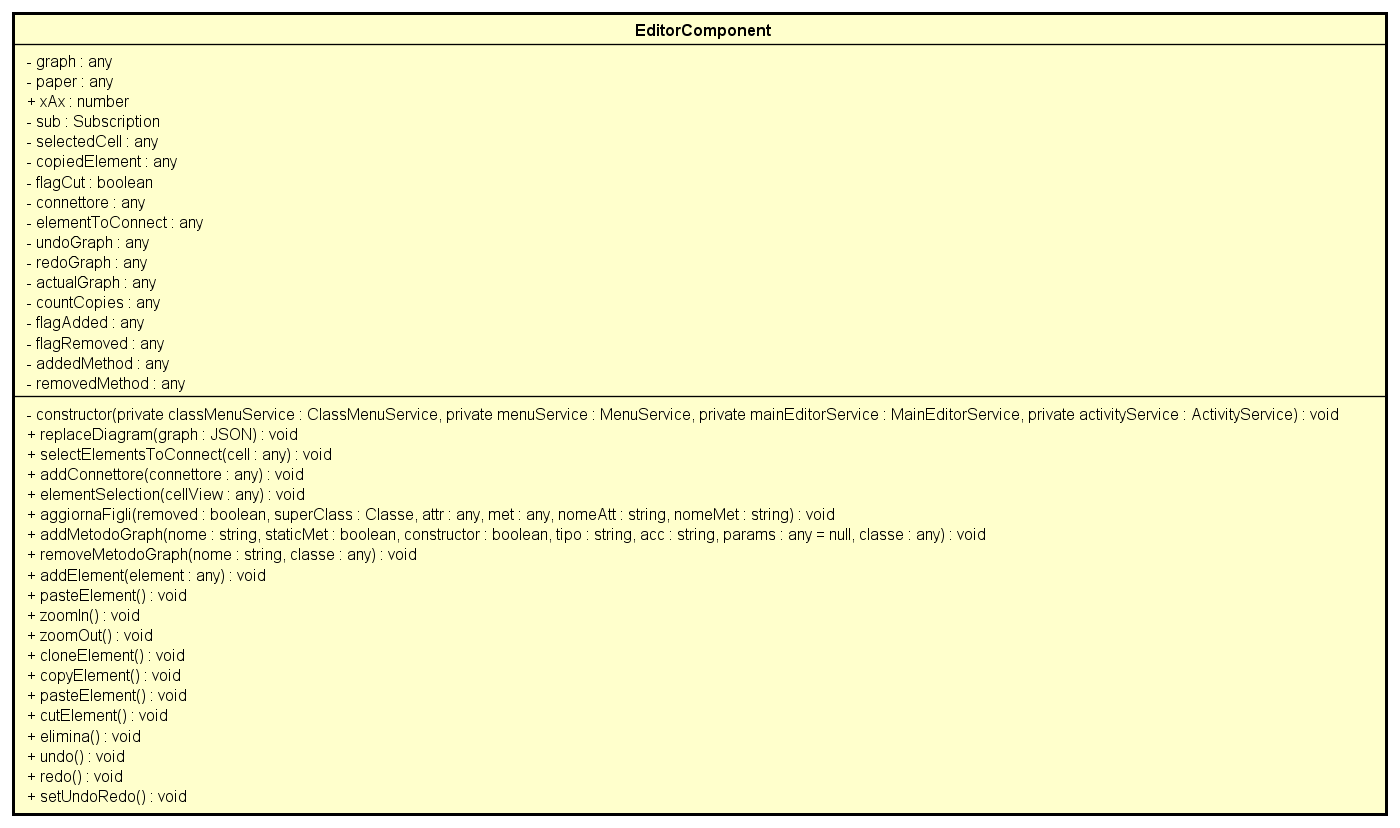
\includegraphics[scale=0.8]{res/sections/SpecificaFrontEnd/Components/Disegnetti/editor.png}
	\caption{Diagramma della classe EditorComponent}
\end{figure}

\begin{itemize}
	\item \textbf{Descrizione:}\\
	Questa classe è il componente principale di gestione dell'editor.
	\item \textbf{Utilizzo:}\\
	Viene utilizzato per la gestione dell'editor.
	\item \textbf{Attributi:}
		\begin{itemize}
			\item \emph{-graph: any}\\
            Contiene tutti gli elementi del grafico
            \item \emph{-paper: any}\\
            Assicura che vengano renderizzati gli elementi del grafico
            \item \emph{+xAx: number}\\
            Serve per scalare il grafico
            \item \emph{-sub: Subscription}\\
            Permette la funzione di zoom
            \item \emph{-selectedCell: any}\\
            Punta all'elemento selezionato con il click
            \item \emph{-copiedElement: any}\\
			Punta all'elemento copiato o tagliato
			\item \emph{-flagCut: boolean}\\
			Indica se l'elemento è stato tagliato, altrimenti è stato copiato
            \item \emph{-connettore: any}\\
            Il tipo del connettore selezionato
            \item \emph{-elementToConnect: any}\\
            Punta all'elemento selezionato con il click, che sarà collegato con il connettore
			\item \emph{-undoGraph: any}\\
			Punta al grafico dopo aver annullato l'ultima operazione
			\item \emph{-redoGraph: any}\\
			Punta al grafico dopo aver ripristinato l'ultima operazione annullata
			\item \emph{-actualGraph: any}\\
			Punta al grafico attuale
			\item \emph{-countCopies: any}\\
			Conta il numero di copie dello stesso elemento
			\item \emph{-flagAdded: any}\\
			Indica se bisogna ascoltare l'evento aggiungere del grafo
			\item \emph{-flagRemoved:any}\\
			Indica se bisogna ascoltare l'evento rimuovere del grafo
			\item \emph{-addedMethod: any}\\
			Indica al metodo annulla se un metodo è stato aggiunto
			\item \emph{-removedMethod: any}\\
			Indica al metodo annulla se un metodo è stato rimosso
		\end{itemize}
	\item \textbf{Metodi:}
		\begin{itemize}
			\item \emph{-constructor(private classMenuService: ClassMenuService, private menuService: MenuService, private mainEditorService: MainEditorService, private activityService: ActivityService)}\\
    		Costruttore della classe\\
    		\textbf{Parametri:}
    		\begin{itemize}
    			\item \emph{classMenuService: ClassMenuService}\\
    			Crea un istanziazione di ClassMenuService
    			\item \emph{menuService: MenuService}\\
    			Crea un istanziazione di MenuService
    			\item \emph{mainEditorService: MainEditorService}\\
    			Crea un istanziazione di MainEditorService
    			\item \emph{activityService: ActivityService}\\
    			Crea un istanziazione di ActivityService
    		\end{itemize}
    		\item \emph{+replaceDiagram(graph: JSON)}\\
    		Rimpiazza l'editor con una nuova finestra contenuta nel file JSON\\
    		\textbf{Parametri:}
    		\begin{itemize}
    			\item \emph{graph: JSON}\\
    			File contenente la finestra
    		\end{itemize}
    		\item \emph{+selectElementsToConnect(cell: any)}\\
    		Seleziona gli elementi da collegare con il connettore\\
    		\textbf{Parametri:}
    		\begin{itemize}
    			\item \emph{cell: any}\\
    			Elemento da collegare
    		\end{itemize}
    		\item \emph{+addConnettore(connettore: any)}\\
    		Aggiunge un connettore alla classe\\
    		\textbf{Parametri:}
    		\begin{itemize}
    			\item \emph{connettore: any}\\
    			Connettore da aggiungere
    		\end{itemize}
    		\item \emph{+elementSelection(cellView: any)}\\
    		Seleziona una shape nell'editor\\
    		\textbf{Parametri:}
    		\begin{itemize}
    			\item \emph{cellView: any}\\
    			Shape da selezionare
    		\end{itemize}
    		\item \emph{+aggiornaFigli(removed: boolean, superClass: Classe, attr: any, met: any, nomeAtt: string, nomeMet: string)}\\
    		Aggiorna i metodi e gli attributi figli della classe padre\\
    		\textbf{Parametri:}
    		\begin{itemize}
    			\item \emph{removed: boolean}\\
    			Indica se deve rimuovere un attributo o un metodo
    			\item \emph{superClass: Classe}\\
    			Classe padre
    			\item \emph{attr: any}\\
    			Attributo da aggiungere
    			\item \emph{met: any}\\
    			Metodo da aggiungere
    			\item \emph{nomeAtt: string}\\
    			Attributo da rimuovere
    			\item \emph{nomeMet: string}\\
    			Metodo da rimuovere
    		\end{itemize}
    		\item \emph{+addMetodoGraph(nome: string, staticMet: boolean, constructor: boolean,
    tipo: string, acc: string, params: any = null, classe: any)}\\
    		Aggiunge alla cella class un metodo\\
    		\textbf{Parametri:}
    		\begin{itemize}
    			\item \emph{nome: string}\\
    			Nome del metodo
    			\item \emph{staticMet: boolean}\\
    			True se è marcato static
    			\item \emph{constructor: boolean}\\
    			True se è un costruttore
    			\item \emph{tipo: string}\\
    			Tipo di ritorno del metodo
    			\item \emph{acc: string}\\
    			Accessibilità del metodo
    			\item \emph{params: any}\\
    			Lista dei parametri del metodo
    			\item \emph{classe: any}\\
    			Indica la cella
    		\end{itemize}
    		\item \emph{+removeMetodoGraph(nome: string, classe: any)}\\
    		Rimuove un metodo dalla cella classe\\
    		\textbf{Parametri:}
    		\begin{itemize}
    			\item \emph{nome: string}\\
    			Nome del metodo
    			\item \emph{classe: any}\\
    			Indica la cella
    		\end{itemize}
    		\item \emph{+addElement(element: any)}\\
    		Aggiunge un elemento all'editor\\
    		\textbf{Parametri:}
    		\begin{itemize}
    			\item \emph{element: any}\\
    			Elemento da aggiungere
    		\end{itemize}
    		\item \emph{+pasteElement()}\\
    		Incolla un elemento precedentemente copiato
    		\item \emph{+zoomIn()}\\
    		Effettua lo zoom in avanti
    		\item \emph{+zoomOut()}\\
    		Effettua lo zoom all'indietro
    		\item \emph{+cloneElement()}\\
    		Clona l'elemento selezionato
    		\item \emph{+copyElement()}\\
    		Copia l'elemento selezionato
    		\item \emph{+pasteElement()}\\
    		Incolla l'elemento precedentemente copiato/tagliato
    		\item \emph{+cutElement()}\\
    		Taglia l'elemento selezionato
    		\item \emph{+elimina()}\\
    		Elimina l'elemento selezionato
    		\item \emph{+undo()}\\
    		Annulla l'ultima azione
    		\item \emph{+redo()}\\
    		Ripristina l'ultima azione annullata
    		\item \emph{+setUndoRedo()}\\
    		Aggiorna il diagramma attuale e il undoGraph
		\end{itemize}
\end{itemize}
				
			\paragraph{SWEDesigner::Client::Components::Editor-container::Editor::Activity-menuComponent}
				\begin{figure}[h!]
	\centering
	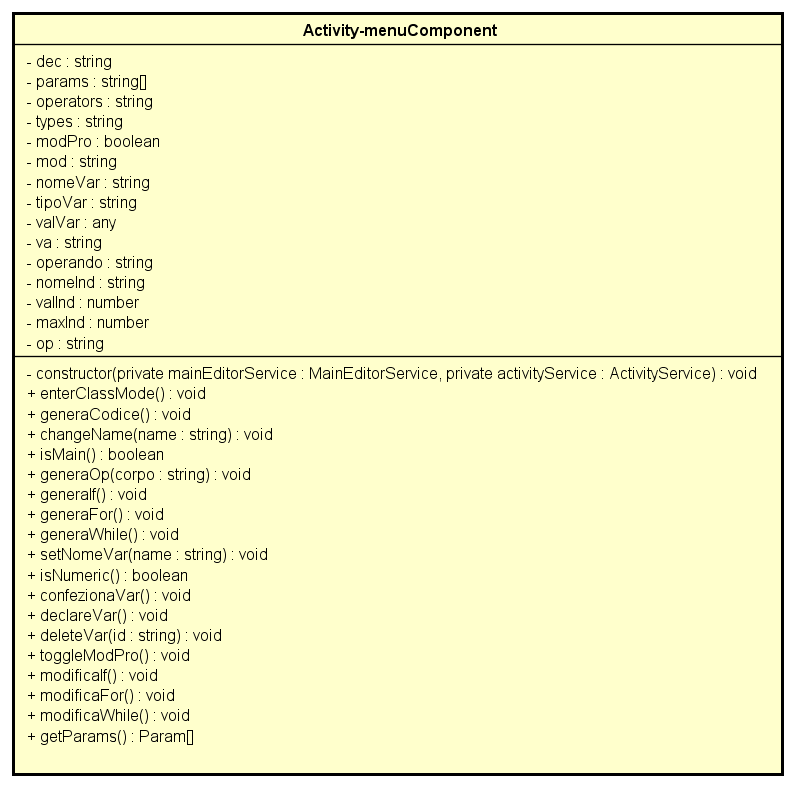
\includegraphics[scale=0.8]{res/sections/SpecificaFrontEnd/Components/Disegnetti/activity-menu.png}
	\caption{Diagramma della classe Activity-menu}
\end{figure}

\begin{itemize}
	
	\item \textbf{Descrizione:}\\
	
	\item \textbf{Utilizzo:}\\
	
	\item \textbf{Attributi:}
		\begin{itemize}
			\item \emph{-decisions: string[]}\\
			
			\item \emph{-dec: string}\\
			
			\item \emph{-params: string[]}\\
			
			\item \emph{-operators: string}\\
			
			\item \emph{-types: string}\\
			
			\item \emph{-modPro: boolean}\\
			
			\item \emph{-mod: string}\\
			
			\item \emph{-nomeVar: string}\\
			
			\item \emph{-tipoVar: string}\\
			
			\item \emph{-valVar: any}\\
			
			\item \emph{-va: string}\\
			
			\item \emph{-operando: string}\\
			
			\item \emph{-nomeInd: string}\\
			
			\item \emph{-valInd: number}\\
			
			\item \emph{-maxInd: number}\\
			
			\item \emph{-op: string}\\
			
		\end{itemize}
	\item \textbf{Metodi:}
		\begin{itemize}
			\item \emph{-constructor(private mainEditorService: MainEditorService,
		private activityService: ActivityService)}\\
    		\\
    		\textbf{Parametri:}
    		\begin{itemize}
    			\item \emph{mainEditorService: MainEditorService}\\
    			
    			\item \emph{activityService: ActivityService}\\
    			
    		\end{itemize}
    		\item \emph{+enterClassMode()}\\
    		
    		\item \emph{+generaCodice()}\\
    		
    		\item \emph{+changeName(name: string)}\\
    		\\
    		\textbf{Parametri:}
    		\begin{itemize}
    			\item \emph{name: string}\\
    			
    		\end{itemize}
    		\item \emph{+isMain()}\\
    		
    		\item \emph{+generaOp(corpo: string)}\\
    		\\
    		\textbf{Parametri:}
    		\begin{itemize}
    			\item \emph{corpo: string}\\
    			
    		\end{itemize}
    		\item \emph{+generaIf()}\\
    		
    		\item \emph{+generaFor()}\\
    		
    		\item \emph{+generaWhile()}\\
    		
    		\item \emph{+setNomeVar(name: string)}\\
    		\\
    		\textbf{Parametri:}
    		\begin{itemize}
    			\item \emph{name: string}\\
    			
    		\end{itemize}
    		\item \emph{+isNumeric()}\\
    		
    		\item \emph{+confezionaVar()}\\
    		
    		\item \emph{+declareVar()}\\
    		
    		\item \emph{+deleteVar(id: string)}\\
    		\\
    		\textbf{Parametri:}
    		\begin{itemize}
    			\item \emph{id: string}\\
    			
    		\end{itemize}
    		\item \emph{+toggleModPro()}\\
    		
    		\item \emph{+modificaIf()}\\
    		
    		\item \emph{+modificaFor()}\\
    		
    		\item \emph{+modificaWhile()}\\
    		
    		\item \emph{+getParams()}\\
    		
		\end{itemize}
\end{itemize}
				
			\paragraph{SWEDesigner::Client::Components::Editor-container::Editor::ToolbarComponent}
				\begin{figure}[h!]
	\centering
	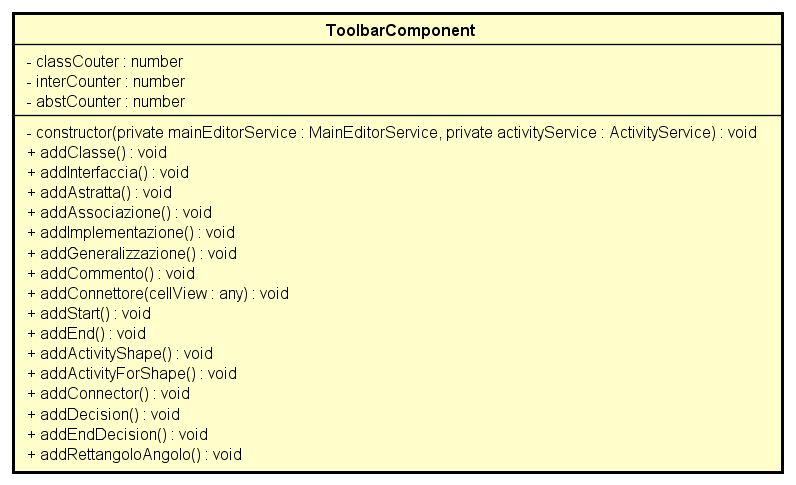
\includegraphics[scale=0.8]{res/sections/SpecificaFrontEnd/Components/Disegnetti/toolbar.png}
	\caption{Diagramma della classe ToolbarComponent}
\end{figure}

\begin{itemize}
	\item \textbf{Descrizione:}\\
	Si occupa della gestione della toolbar.
	\item \textbf{Utilizzo:}\\
	Viene usato dall'EditorComponent per la gestione della toolbar.
	\item \textbf{Attributi:}
		\begin{itemize}
			\item \emph{-classCouter: number}\\
			Conta il numero di classi presenti nell'editor
			\item \emph{-interCounter: number}\\
			Conta il numero di interfacce presenti nell'editor
			\item \emph{-abstCounter: number}\\
			Conta il numero di classi astratte presenti nell'editor
		\end{itemize}
	\item \textbf{Metodi:}
		\begin{itemize}
			\item \emph{-constructor(private mainEditorService: MainEditorService, private activityService: ActivityService)}\\
    		Costruttore della classe\\
    		\textbf{Parametri:}
    		\begin{itemize}
    			\item \emph{mainEditorService: MainEditorService}\\
    			Crea un istanziazione di MainEditorService
    			\item \emph{activityService: ActivityService}\\
    			Crea un istanziazione di AcrivityService
    		\end{itemize}
    		\item \emph{+addClasse()}\\
    		Aggiunge una classe all'editor
    		\item \emph{+addInterfaccia()}\\
    		Aggiunge un interfaccia all'editor
    		\item \emph{+addAstratta()}\\
    		Aggiunge una classe astratta all'editor
    		\item \emph{+addAssociazione()}\\
    		Seleziona il tipo di connettore \textit{Associazione}
    		\item \emph{+addImplementazione()}\\
    		Seleziona il tipo di connettore \textit{Implementazione}
    		\item \emph{+addGeneralizzazione()}\\
    		Seleziona il tipo di connettore \textit{Generalizzazione}
    		\item \emph{+addCommento()}\\
    		Aggiunge un commento all'editor
    		\item \emph{+addConnettore(cellView: any)}\\
    		Aggiunge il connettore selezionato
    		\begin{itemize}
    			\item \emph{cellView: any}\\
    			Elemento target o source
    		\end{itemize}
    		\item \emph{+addStart()}\\
    		Aggiunge l'elemento start all'editor
    		\item \emph{+addEnd()}\\
    		Aggiunge l'elemento end all'editor
    		\item \emph{+addActivityShape()}\\
    		Aggiunge un azione
    		\item \emph{+addConnector()}\\
    		Seleziona il connettore freccia per l'activity diagram
    		\item \emph{+addDecision()}\\
    		Aggiunge all'editor un inizio if/ciclo
    		\item \emph{+addEndDecision()}\\
    		Aggiunge all'editor una fine if/ciclo
    		\item \emph{+addRettangoloAngolo()}\\
    		Aggiunge un attività
		\end{itemize}
\end{itemize}
				
			\paragraph{SWEDesigner::Client::Components::Editor-container::Editor::ActivityService}
				\begin{figure}[h!]
	\centering
	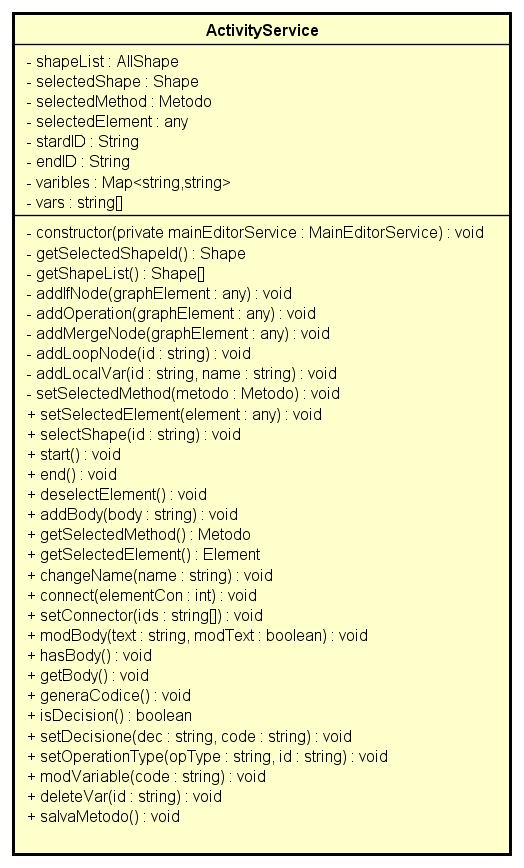
\includegraphics[scale=0.8]{res/sections/SpecificaFrontEnd/Services/Disegnetti/activity.png}
	\caption{Diagramma della classe ActivityService}
\end{figure}

\begin{itemize}
	\item \textbf{Descrizione:}\\
	
	\item \textbf{Utilizzo:}\\
	
	\item \textbf{Attributi:}
		\begin{itemize}
			\item \emph{-shapeList:AllShape}\\
			Lista della shape
			\item \emph{-selectedShape: Shape}\\
			Shape selezionata
			\item \emph{-selectedMethod: Metodo}\\
			Metodo selezionato
			\item \emph{-selectedElement: any}\\
			Elemento selezionato
			\item \emph{-stardID: string}\\
			Id dell'elemento start
			\item \emph{-endID: string}\\
			Id dell'elemento end
			\item \emph{-varibles: Map<string, string>}\\
			Lista dei parametri
			\item \emph{-vars: string[]}\\
			Lista delle variabili
		\end{itemize}
	\item \textbf{Metodi:}
		\begin{itemize}
			\item \emph{-constructor(private mainEditorService: MainEditorService}\\
    		Costruttore della classe\\
    		\textbf{Parametri:}
    		\begin{itemize}
    			\item \emph{mainEditorService: MainEditorService}\\
    			Crea un istanziazione di MainEditorService
    		\end{itemize}
    		\item \emph{-getSelectedShapeId()}\\
    		Ritorna l'id della shape selezionata
    		\item \emph{-getShapeList()}\\
    		Ritorna la lista della shapes
    		\item \emph{-addIfNode(graphElement: any)}\\
    		Aggiunge un if statement\\
    		\textbf{Parametri:}
    		\begin{itemize}
    			\item \emph{graphElement: any}\\
    			Si riferisce al diagramma
    		\end{itemize}
    		\item \emph{-addOperation(graphElement: any)}\\
    		Aggiunge un operazione\\
    		\textbf{Parametri:}
    		\begin{itemize}
    			\item \emph{graphElement: any}\\
    			Si riferisce al diagramma
    		\end{itemize}
    		\item \emph{-addMergeNode(graphElement: any)}\\
    		Aggiunge un merge\\
    		\textbf{Parametri:}
    		\begin{itemize}
    			\item \emph{graphElement: any}\\
    			Si riferisce al diagramma
    		\end{itemize}
    		\item \emph{-addLoopNode(id: string)}\\
    		Aggiunge un ciclo\\
    		\textbf{Parametri:}
    		\begin{itemize}
    			\item \emph{id: string}\\
    			Id della shape
    		\end{itemize}
    		\item \emph{-addLocalVar(id: string, name: string)}\\
    		Aggiunge una variabile locale\\
    		\textbf{Parametri:}
    		\begin{itemize}
    			\item \emph{id: string}\\
    			Id della shape
    			\item \emph{name: string}\\
    			Nome della variabile
    		\end{itemize}
    		\item \emph{-setSelectedMethod(metodo: Metodo)}\\
    		Setta il metodo selezionato\\
    		\textbf{Parametri:}
    		\begin{itemize}
    			\item \emph{metodo: Metodo}\\
    			Metodo da selezionare
    		\end{itemize}
    		\item \emph{+setSelectedElement(element: any)}\\
    		Setta l'elemento selezionato\\
    		\textbf{Parametri:}
    		\begin{itemize}
    			\item \emph{element: any}\\
    			Elemento selezionato
    		\end{itemize}
    		\item \emph{+selectShape(id: string)}\\
    		Seleziona la shape\\
    		\textbf{Parametri:}
    		\begin{itemize}
    			\item \emph{id: string}\\
    			Id della shape da seleionare
    		\end{itemize}
    		\item \emph{+start()}\\
    		Permette di aggiunger una shape start
    		\item \emph{+end()}\\
    		Permette di aggiungere una shape end
    		\item \emph{+deselectElement()}\\
    		Deseleziona l'elemento
    		\item \emph{+addBody(body: string)}\\
    		Aggiunge il body della shape\\
    		\textbf{Parametri:}
    		\begin{itemize}
    			\item \emph{body: string}\\
    			Body della shape
    		\end{itemize}
    		\item \emph{+getSelectedMethod()}\\
    		Ritorna il metodo selezionato
    		\item \emph{+getSelectedElement()}\\
    		Ritorna l'elemento selezionato
    		\item \emph{+getNameMethod()}\\
    		Ritorna il nome del metodo
    		\item \emph{+getVarVis()}\\
    		Ritorna il valore di vars
    		\item \emph{+getShapeType()}\\
    		Ritorna il tipo della shape
    		\item \emph{+changeName(name:string)}\\
    		Modifica il nome della shape\\
    		\textbf{Parametri:}
    		\begin{itemize}
    			\item \emph{name: string}\\
    			Nuovo nome della shape
    		\end{itemize}
    		\item \emph{+connect(elementCon: any)}\\
    		Linka la shape\\
    		\textbf{Parametri:}
    		\begin{itemize}
    			\item \emph{elementCon: any}\\
    			Shape da linkare
    		\end{itemize}
    		\item \emph{+setConnector(ids: string[])}\\
    		Connette la shape\\
    		\textbf{Parametri:}
    		\begin{itemize}
    			\item \emph{ids: string[]}\\
    			Id della shape da connettere
    		\end{itemize}
    		\item \emph{+modBody(text: string, modText: boolean)}\\
    		Modifica il body della shape\\
    		\textbf{Parametri:}
    		\begin{itemize}
    			\item \emph{text: string}\\
    			Nuovo valore
    			\item \emph{modText: boolean}\\
    			Nuovo valore
    		\end{itemize}
    		\item \emph{+hasBody()}\\
    		Controlla se ha un body
    		\item \emph{+getBody()}\\
    		Restituisce il body
    		\item \emph{+generaCodice()}\\
    		Genera il codice
    		\item \emph{+isDecision()}\\
    		True se è una decisione
    		\item \emph{+isVarDeclaration()}\\
    		True se è una dichiarazione
    		\item \emph{+setDecisione(dec: string, code: string)}\\
    		Setta il nuovo valore della decisione\\
    		\textbf{Parametri:}
    		\begin{itemize}
    			\item \emph{dec: string}\\
    			Nuovo valore
    			\item \emph{code: string}\\
    			Codice
    		\end{itemize}
    		\item \emph{+setOperationType(opType: string, id: string)}\\
    		Setta il tipo di operazione\\
    		\textbf{Parametri:}
    		\begin{itemize}
    			\item \emph{opType: string}\\
    			Tipo di operazione
    			\item \emph{id: string}\\
    			Id della shape
    		\end{itemize}
    		\item \emph{+modVariable(code: string)}\\
    		Setta il nuovo valore della variabile\\
    		\textbf{Parametri:}
    		\begin{itemize}
    			\item \emph{code: string}\\
    			Nuovo valore
    		\end{itemize}
    		\item \emph{+deleteVar(id: string)}\\
    		Elimina una variabile\\
    		\textbf{Parametri:}
    		\begin{itemize}
    			\item \emph{id: string}\\
    			Id della variabile da eliminare
    		\end{itemize}
    		\item \emph{+salvaMetodo()}\\
    		Salva il metodo
		\end{itemize}
\end{itemize}
				
			\paragraph{SWEDesigner::Client::Components::Editor-container::Editor::Class-menuService}
				\begin{figure}[h!]
	\centering
	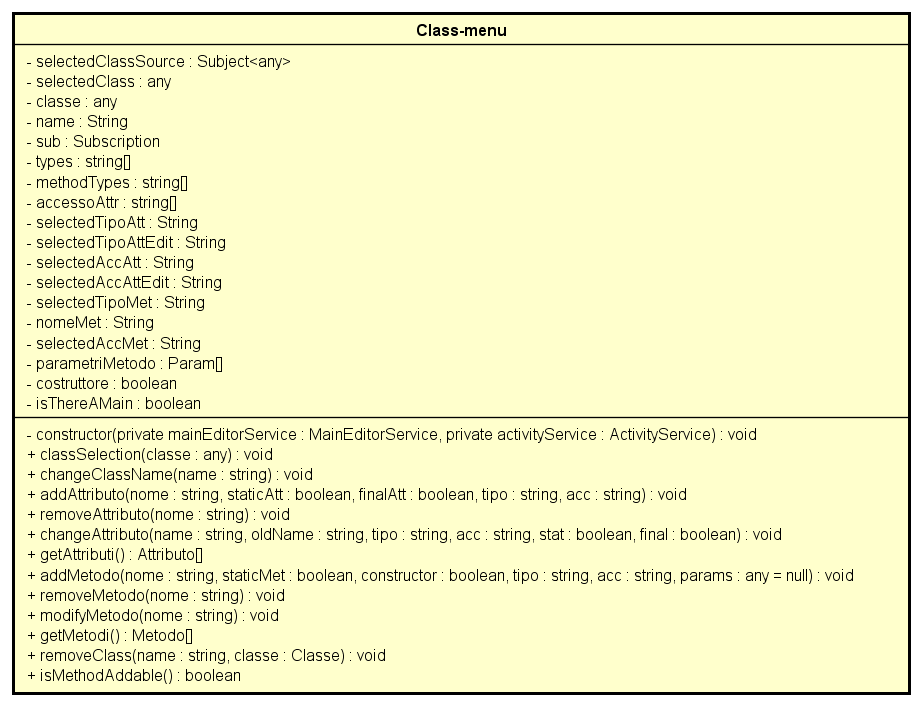
\includegraphics[scale=0.8]{res/sections/SpecificaFrontEnd/Services/Disegnetti/class-menu.png}
	\caption{Diagramma della classe Class-menu}
\end{figure}

\begin{itemize}
	\item \textbf{Descrizione:}\\
	
	\item \textbf{Utilizzo:}\\
	
	\item \textbf{Attributi:}
		\begin{itemize}
			\item \emph{-selectedClassSource: Subject<any>}\\
			Risorsa observable oggetto-classe
			\item \emph{-selectedClass: any}\\
			Stream observable oggetto-classe
			\item \emph{-classe: any}\\
			La classe correntemente selezionata nell'editor
			\item \emph{-name: string}\\
			Il nome della classe correntemente selezionata nell'editor
			\item \emph{-sub: Subscription}\\
			Subscription dell'oggetto observable che è la classe selezionata nell'editor
			\item \emph{-types: string[]}\\
			Array di tipi di dato primitivi
			\item \emph{-methodTypes: string[]}\\
			Array di tipi di dato primitivi per i tipi di ritorno dei metodi
			\item \emph{-accessoAttr: string[]}\\
			Array contenente le visibilità delle classi
			\item \emph{-selectedTipoAtt: string}\\
			Usato per memorizzare il tipo selezionato per il costruttore di un nuovo attributo
			\item \emph{-selectedTipoAttEdit: string}\\
			Usato per memorizzare il tipo selezionato per editare l'attributo
			\item \emph{-selectedAccAtt: String}\\
			Usato per memorizzare la visibilità selezionata per costruire un nuovo attributo
			\item \emph{-selectedAccAttEdit: String}\\
			Usato per memorizzare la visibilità selezionata per editare l'attributo
			\item \emph{-selectedTipoMet: String}\\
			Usato per memorizzare il tipo di ritorno selezionato per costruire un nuovo metodo
			\item \emph{-nomeMet: String}\\
			Usato per memorizzare il nome del nuovo metodo
			\item \emph{-selectedAccMet: String}\\
			Usato per selezionare la visibilità per costruire un nuovo metodo
			\item \emph{-parametriMetodo: Param[]}\\
			Usato per memorizzare un array di parametri per costruire un nuovo metodo
			\item \emph{-costruttore: boolean}\\
			Usato per memorizzare se il metodo è un costruttore
			\item \emph{-isThereAMain: boolean}\\
			Usato per memorizzare se è stato aggiunto il metodo main
		\end{itemize}
	\item \textbf{Metodi:}
		\begin{itemize}
			\item \emph{-constructor(private mainEditorService: MainEditorService,
    private activityService: ActivityService)}\\
    		Crea un istanziazione di ClassMenuComponent e setta le proprietà classe e nome per subscription da classMenuService\\
    		\textbf{Parametri:}
    		\begin{itemize}
    			\item \emph{mainEditorService: MainEditorService}\\
    			Usato per creare una nuova istanziazione di ClassMenuService
    			\item \emph{activityService: ActivityService}\\
    			Usato per creare una nuova istanziazione di ClassMenuService
    		\end{itemize}
    		\item \emph{+classSelection(classe: any)}\\
    		Comandi messaggio del servizio\\
    		\textbf{Parametri:}
    		\begin{itemize}
    			\item \emph{classe: any}\\
    			Variabile usata per settare la classe selezionata
    		\end{itemize}
    		\item \emph{+changeClassName(name: string)}\\
    		Cambia il nome della classe selezionata\\
    		\textbf{Parametri:}
    		\begin{itemize}
    			\item \emph{name: string}\\
    			Nuovo nome della classe
    		\end{itemize}
    		\item \emph{+addAttributo(nome: string, staticAtt: boolean, finalAtt: boolean, tipo: string, acc: string)}\\
    		Aggiunge un nuovo attributo alla classe\\
    		\textbf{Parametri:}
    		\begin{itemize}
    			\item \emph{nome: string}\\
    			Nome dell'attributo
    			\item \emph{staticAtt: boolean}\\
    			True se l'attributo è static
    			\item \emph{finalAtt: boolean}\\
    			True se l'attributo è final
    			\item \emph{tipo: string}\\
    			Tipo dell'attributo
    			\item \emph{acc: string}\\
    			Visibilità dell'attributo
    		\end{itemize}
    		\item \emph{+removeAttributo(nome: string)}\\
    		Rimuove un attributo dalla classe selezionata\\
    		\textbf{Parametri:}
    		\begin{itemize}
    			\item \emph{nome: string}\\
    			Nome dell'attributo da rimuovere
    		\end{itemize}
    		\item \emph{+changeAttributo(name: string, oldName: string, tipo: string, acc: string , stat: boolean, final: boolean)}\\
    		Modifica le proprietà di un attributo della classe selezionata\\
    		\textbf{Parametri:}
    		\begin{itemize}
    			\item \emph{name: string}\\
    			Nuovo nome dell'attributo
    			\item \emph{oldName: string}\\
    			Vecchio nome dell'attribuo
    			\item \emph{tipo: string}\\
    			Tipo dell'attributo
    			\item \emph{acc: string}\\
    			Tipo di visibilità
    			\item \emph{stat: boolean}\\
    			True se è marcato static
    			\item \emph{final: boolean}\\
    			True se è marcato final
    		\end{itemize}
    		\item \emph{+getAttributi()}\\
    		Ritorna la lista degli attributi di una classe
    		\item \emph{+addMetodo(nome: string, staticMet: boolean, constructor: boolean, tipo: string, acc: string, params: any = null)}\\
    		Aggiunge un nuovo metodo alla classe selezionata\\
    		\textbf{Parametri:}
    		\begin{itemize}
    			\item \emph{nome: string}\\
    			Nome del metodo
    			\item \emph{staticMet: boolean}\\
    			True se è marcato static
    			\item \emph{constructor: boolean}\\
    			True se è un costruttore
    			\item \emph{tipo: string}\\
    			Tipo del metodo
    			\item \emph{acc: string}\\
    			Visibilità del metodo
    			\item \emph{params: any = null}\\
    			Lista di parametri del metodo
    		\end{itemize}
    		\item \emph{+removeMetodo(nome: string)}\\
    		Rimuove un metodo dalla classe selezionata\\
    		\textbf{Parametri:}
    		\begin{itemize}
    			\item \emph{nome: string}\\
    			Nome del metodo da rimuovere
    		\end{itemize}
    		\item \emph{+modifyMetodo(nome: string)}\\
    		Setta la modalità activity nell'editor per editare il metodo della classe selezionata\\
    		\textbf{Parametri:}
    		\begin{itemize}
    			\item \emph{nome: string}\\
    			Nome del metodo da editare
    		\end{itemize}
    		\item \emph{+getMetodi()}\\
    		Ritorna la lista dei metodi di una classe
    		\item \emph{+removeClass(name: string, classe: Classe)}\\
    		Rimuove la classe selezionata\\
    		\textbf{Parametri:}
    		\begin{itemize}
    			\item \emph{name: string}\\
    			Nome della classe
    			\item \emph{classe: Classe}\\
    			Tipo della classe
    		\end{itemize}
    		\item \emph{+isMethodAddable()}\\
    		Ritorna true se il metodo è aggiungibile dalla logica
		\end{itemize}
\end{itemize}
				
			\paragraph{SWEDesigner::Client::Components::Editor-container::Editor::All-shape}
				\begin{figure}[h!]
	\centering
	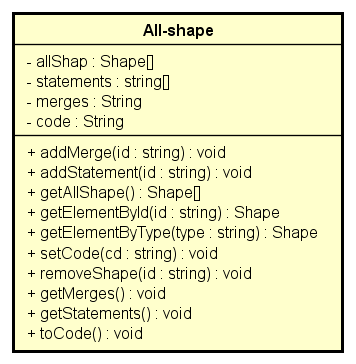
\includegraphics[scale=0.8]{res/sections/SpecificaFrontEnd/Services/Disegnetti/all-shape.png}
	\caption{Diagramma della classe All-shape}
\end{figure}

\begin{itemize}
	\item \textbf{Descrizione:}\\
	
	\item \textbf{Utilizzo:}\\
	
	\item \textbf{Attributi:}
		\begin{itemize}
			\item \emph{-allShap: Shape[]}\\
			Rappresenta l'array di shapes
			\item \emph{-statements: string[]}\\
			Rappresenta lo stato delle shapes
			\item \emph{-merges: string}\\
			Ritorna il risultato delle shapes mergiate
			\item \emph{-code: string}\\
			Contiene il codice generato dal metodo
		\end{itemize}
	\item \textbf{Metodi:}
		\begin{itemize}
			\item \emph{+addMerge(id: string)}\\
    		Aggiunge il codice corrente al progetto\\
    		\textbf{Parametri:}
    		\begin{itemize}
    			\item \emph{id: string}\\
    			Progetto
    		\end{itemize}
    		\item \emph{+addStatement(id: string)}\\
    		Aggiunge lo statement alla decisione\\
    		\textbf{Parametri:}
    		\begin{itemize}
    			\item \emph{id: string}\\
    			Statement da aggiungere
    		\end{itemize}
    		\item \emph{+getAllShape()}\\
    		Ritorna tutte le shapes
    		\item \emph{+getElementById(id: string)}\\
    		Ritorna il riferimento alla shape selezionata\\
    		\textbf{Parametri:}
    		\begin{itemize}
    			\item \emph{id: string}\\
    			Shape selezionata
    		\end{itemize}
    		\item \emph{+getElementByType(type: string)}\\
    		Ritorna il riferimento alla shape selezionata\\
    		\textbf{Parametri:}
    		\begin{itemize}
    			\item \emph{type: string}\\
    			Shape eselzionata
    		\end{itemize}
    		\item \emph{+setCode(cd: string)}\\
    		Setta la variabile code con il nuovo valore\\
    		\textbf{Parametri:}
    		\begin{itemize}
    			\item \emph{cd: string}\\
    			Nuovo valore
    		\end{itemize}
    		\item \emph{+removeShape(id: string)}\\
    		Rimuove la shape selezionata\\
    		\textbf{Parametri:}
    		\begin{itemize}
    			\item \emph{id: string}\\
    			Shape da rimuovere
    		\end{itemize}
    		\item \emph{+getMerges()}\\
    		Ritorna l'attributo merges
    		\item \emph{+getStatements()}\\
    		Ritorna l'attributo statements
    		\item \emph{+toCode()}\\
    		Converte le shape in codice
		\end{itemize}
\end{itemize}
				
			\paragraph{SWEDesigner::Client::Components::Editor-container::Editor::Attributo}
				\begin{figure}[h!]
	\centering
	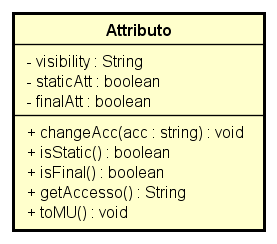
\includegraphics[scale=0.8]{res/sections/SpecificaFrontEnd/Services/Disegnetti/attributo.png}
	\caption{Diagramma della classe Attributo}
\end{figure}

\begin{itemize}
	\item \textbf{Descrizione:}\\
	Modello che contiene tutti i dati relativi al salvataggio di un attributo
	\item \textbf{Utilizzo:}\\
	Utilizzato per salvare i dati di un attributo.
	\item \textbf{Attributi:}
		\begin{itemize}
			\item \emph{-visibility: string}\\
			Visibilità dell'attributo
			\item \emph{-staticAtt: boolean}\\
			True se è marcato static
			\item \emph{-finalAtt: boolean}\\
			True se è marcato final
		\end{itemize}
	\item \textbf{Metodi:}
		\begin{itemize}
			\item \emph{+changeAcc(acc: string)}\\
    		Modifica la visibilità dell'attributo\\
    		\textbf{Parametri:}
    		\begin{itemize}
    			\item \emph{acc: string}\\
    			Nuova visibilità dell'attributo
    		\end{itemize}
    		\item \emph{+isStatic()}\\
    		Ritorna true se l'attributo è statico
    		\item \emph{+isFinal()}\\
    		Ritorna true se l'attributo è final
    		\item \emph{+getAccesso()}\\
    		Ritorna la visibilità dell'attributo
    		\item \emph{+toMU()}\\
    		Converte l'attributo in una stringa o un file JSON
    	\end{itemize}
\end{itemize}
				
			\paragraph{SWEDesigner::Client::Components::Editor-container::Editor::Class-errors}
				\input{res/sections/SpecificaFrontEnd/Services/class-errors.tex}
				
			\paragraph{SWEDesigner::Client::Components::Editor-container::Editor::Classe-astratta}
				\begin{figure}[h!]
	\centering
	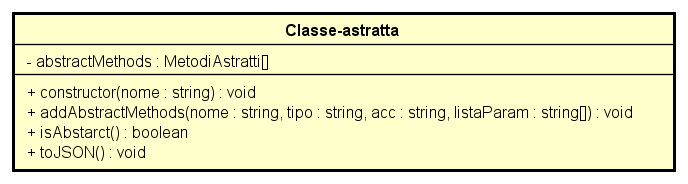
\includegraphics[scale=0.8]{res/sections/SpecificaFrontEnd/Services/Disegnetti/classe-astratta.png}
	\caption{Diagramma della classe Classe-astratta}
\end{figure}

\begin{itemize}
	\item \textbf{Descrizione:}\\
	
	\item \textbf{Utilizzo:}\\
	
	\item \textbf{Attributi:}
		\begin{itemize}
			\item \emph{-abstractMethods: MetodiAstratti[]}\\
			Array contenente i metodi della classe astratta
		\end{itemize}
	\item \textbf{Metodi:}
		\begin{itemize}
			\item \emph{+constructor(nome: string)}\\
    		Costruttore della classe astratta\\
    		\textbf{Parametri:}
    		\begin{itemize}
    			\item \emph{nome: string}\\
    			Nome della classe astratta da creare
    		\end{itemize}
    		\item \emph{+addAbstractMethods(nome: string, tipo: string, acc:string, listaParam: string[])}\\
    		Aggiunge un metodo astratto alla classe\\
    		\textbf{Parametri:}
    		\begin{itemize}
    			\item \emph{nome: string}\\
    			Nome del metodo
    			\item \emph{tipo: string}\\
    			Tipo di ritorno del metodo
    			\item \emph{acc:string}\\
    			Visibilità del metodo
    			\item \emph{listaParam: string[]}\\
    			Lista dei parametri del metodo
    		\end{itemize}
    		\item \emph{+isAbstarct()}\\
    		Ritorna true se l'oggetto è astratto
    		\item \emph{+toJSON()}\\
    		Parsa la classe selezionata e la trasforma in formato JSON
    	\end{itemize}
\end{itemize}
				
			\paragraph{SWEDesigner::Client::Components::Editor-container::Editor::Classe}
				\begin{itemize}
	\item \textbf{Descrizione:}\\
	
	\item \textbf{Utilizzo:}\\
	
	\item \textbf{Attributi:}
		\begin{itemize}
			\item \emph{-nome: string}\\
			Nome della classe, usato come identificatore
			\item \emph{-attributi: Attributo[]}\\
			Lista degli attributi della classe
			\item \emph{-metodi: Metodo[]}\\
			Lista dei metodi della classe
			\item \emph{-classePadre: string}\\
			Nome della classe estesa da questa classe
		\end{itemize}
	\item \textbf{Metodi:}
		\begin{itemize}
			\item \emph{-constructor(nome: string)}\\
    		Costruisce la classe\\
    		\textbf{Parametri:}
    		\begin{itemize}
    			\item \emph{nome: string}\\
    			Nome della classe da costruire
    		\end{itemize}
    		\item \emph{+addAttributo(tipo: string, nome: string, acc: string, stat: boolean, fin: boolean)}\\
    		Aggiunge un nuovo attributo all'array di attributi della classe selezionata\\
    		\textbf{Parametri:}
    		\begin{itemize}
    			\item \emph{tipo: string}\\
    			Tipo dell'attributo
    			\item \emph{nome: string}\\
    			Nome dell'attributo
    			\item \emph{acc: string}\\
    			Visibilità dell'attributo
    			\item \emph{stat: boolean}\\
    			True se è marcato static
    			\item \emph{fin: boolean}\\
    			True se è marcato finale
    		\end{itemize}
    		\item \emph{+addSuperclass(superclass: string)}\\
    		Aggiunge il nome della classe che è estesa da questa classe\\
    		\textbf{Parametri:}
    		\begin{itemize}
    			\item \emph{superclass: string}\\
    			Nome della superclasse
    		\end{itemize}
    		\item \emph{+addMetodo(metodo: Metodo) }\\
    		Aggiunge un metodo alla classe selezionata\\
    		\textbf{Parametri:}
    		\begin{itemize}
    			\item \emph{metodo: Metodo}\\
    			Metodo da aggiungere
    		\end{itemize}
    		\item \emph{+changeNome(name: string)}\\
    		Modifica il nome della classe selezionata\\
    		\textbf{Parametri:}
    		\begin{itemize}
    			\item \emph{name: string}\\
    			Nuovo nome della classe
    		\end{itemize}
    		\item \emph{+changeAttr(nomeAttr: string, tipo: string, nuovoNome: string, acc: string)}\\
    		Modifica un attributo della classe selezionata\\
    		\textbf{Parametri:}
    		\begin{itemize}
    			\item \emph{nomeAttr: string}\\
    			Vecchio nome dell'attributo
    			\item \emph{tipo: string}\\
    			Tipo dell'attributo
    			\item \emph{nuovoNome: string}\\
    			Nuovo nome dell'attributo
    			\item \emph{acc: string}\\
    			Accessibilità dell'attributo
    		\end{itemize}
    		\item \emph{+removeAttr(nomeAttr: string)}\\
    		Rimuove un attributo dalla lista degli attributi della classe\\
    		\textbf{Parametri:}
    		\begin{itemize}
    			\item \emph{nomeAttr: string}\\
    			Nome dell'attributo da rimuovere
    		\end{itemize}
    		\item \emph{+removeMetodo(nomeMetodo: string)}\\
    		Rimuove un metodo dalla lista dei metodi della classe\\
    		\textbf{Parametri:}
    		\begin{itemize}
    			\item \emph{nomeMetodo: string}\\
    			Nome del meotodo da rimuovere
    		\end{itemize}
    		\item \emph{+getSottoclasse() }\\
    		Ritorna il nome della superclasse
    		\item \emph{+isInterface()}\\
    		Ritorna true se l'oggetto è un interfaccia
    		\item \emph{+isAbstract()}\\
    		Ritorna true se l'oggetto è astratto
    		\item \emph{+getNome()}\\
    		Ritorna il nome della classe
    		\item \emph{+getAttributi()}\\
    		Ritorna la lista degli attributi della classe
    		\item \emph{+getMetodi()}\\
    		Ritorna la lista dei metodi della classe
    		\item \emph{+retriveMethod(name: string)}\\
    		Ritorna un determinato metodo dall'array dei metodi\\
    		\textbf{Parametri:}
    		\begin{itemize}
    			\item \emph{name: string}\\
    			Nome del metodo da ritornare
    		\end{itemize}
    		\item \emph{+toJSON()}\\
    		Effettua override della funzione 
    		\item \emph{+retrievePublicAttr()}\\
    		
    		\item \emph{+retrievePrivateAttr()}\\
    		
    		\item \emph{+toMU()}\\
    		
    		\item \emph{+getInfoPublic(x: any)}\\
    		\\
    		\textbf{Parametri:}
    		\begin{itemize}
    			\item \emph{x: any}\\
    			
    		\end{itemize}
    		\item \emph{+getInfoPrivate(x)}\\
    		\\
    		\textbf{Parametri:}
    		\begin{itemize}
    			\item \emph{x: any}\\
    			
    		\end{itemize}
    	\end{itemize}
\end{itemize}
				
			\paragraph{SWEDesigner::Client::Components::Editor-container::Editor::Elemento-metodo}
				\input{res/sections/SpecificaFrontEnd/Services/elemento-metodo.tex}
				
			\paragraph{SWEDesigner::Client::Components::Editor-container::Editor::End}
				\begin{figure}[h!]
	\centering
	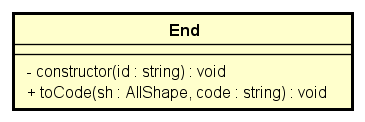
\includegraphics[scale=0.8]{res/sections/SpecificaFrontEnd/Services/Disegnetti/end.png}
	\caption{Diagramma della classe End}
\end{figure}

\begin{itemize}
	\item \textbf{Descrizione:}\\
	
	\item \textbf{Utilizzo:}\\
	
	\item \textbf{Metodi:}
		\begin{itemize}
			\item \emph{-constructor(id : string)}\\
    		\\
    		\textbf{Parametri:}
    		\begin{itemize}
    			\item \emph{id : string}\\
    			
    		\end{itemize}
			\item \emph{+getType())}\\
    		
			\item \emph{+toCode(sh: AllShape, code: string)}\\
    		\\
    		\textbf{Parametri:}
    		\begin{itemize}
    			\item \emph{sh: AllShape}\\
    			
    			\item \emph{code: string}\\
    			
    		\end{itemize}
    	\end{itemize}
\end{itemize}
				
			\paragraph{SWEDesigner::Client::Components::Editor-container::Editor::If-node}
				\begin{itemize}
	\item \textbf{Descrizione:}\\
	
	\item \textbf{Utilizzo:}\\
	
	\item \textbf{Attributi:}
		\begin{itemize}
			\item \emph{-succElse: string}\\
			
		\end{itemize}
	\item \textbf{Metodi:}
		\begin{itemize}
			\item \emph{-constructor(id: string)}\\
    		\\
    		\textbf{Parametri:}
    		\begin{itemize}
    			\item \emph{id: string}\\
    			
    		\end{itemize}
    		\item \emph{+getSuccElse()}\\
    		
    		\item \emph{+setSuccElse(succElse: string)}\\
    		\\
    		\begin{itemize}
    			\item \emph{succElse: string}\\
    			
    		\end{itemize}
    		\item \emph{+getType()}\\
    		
    		\item \emph{+toCode(sh: AllShape, code: string)}\\
    		\\
    		\textbf{Parametri:}
    		\begin{itemize}
    			\item \emph{sh: AllShape}\\
    			
    			\item \emph{code: string}\\
    			
    		\end{itemize}
    	\end{itemize}
\end{itemize}
				
			\paragraph{SWEDesigner::Client::Components::Editor-container::Editor::Interface}
				\begin{itemize}
	\item \textbf{Descrizione:}\\
	
	\item \textbf{Utilizzo:}\\
	
	\item \textbf{Metodi:}
		\begin{itemize}
			\item \emph{-constructor(nome: string)}\\
    		Costruisce una nuova interfaccia\\
    		\textbf{Parametri:}
    		\begin{itemize}
    			\item \emph{nome: string}\\
    			Nome dell'interfaccia
    		\end{itemize}
    		\item \emph{+addAttributo(tipo: string, nome: string, acc: string, stat: boolean, fin: boolean)}\\
    		Aggiunge un attributo all'array di attributi dell'interfaccia\\
    		\textbf{Parametri:}
    		\begin{itemize}
    			\item \emph{tipo: string}\\
    			Tipo dell'attributo
    			\item \emph{nome: string}\\
    			Nome dell'attributo
    			\item \emph{acc: string}\\
    			Visibilità dell'attributo
    			\item \emph{stat: boolean}\\
    			True se è marcato static
    			\item \emph{fin: boolean}\\
    			True se è marcato final
    		\end{itemize}
    		\item \emph{+addMetodo(metodo: Metodo)}\\
    		Aggiunge un metodo all'array di metodi dell'interfaccia\\
    		\textbf{Parametri:}
    		\begin{itemize}
    			\item \emph{metodo: Metodo}\\
    			Netodo da aggiungere
    		\end{itemize}
    		\item \emph{+changeAttr(nomeAttr: string, tipo: string, nuovoNome: string, acc: string)}\\
    		Modifica un attributo dell'interfaccia\\
    		\textbf{Parametri:}
    		\begin{itemize}
    			\item \emph{nomeAttr: string}\\
    			Vecchio nome dell'attributo
    			\item \emph{tipo: string}\\
    			Tipo dell'attributo
    			\item \emph{nuovoNome: string}\\
    			Nuovo nome dell'attributo
    			\item \emph{acc: string}\\
    			Visibilità dell'attributo
    		\end{itemize}
    		\item \emph{+removeAttr(nomeAttr: string)}\\
    		Rimuove un attributo dalla lista degli attributi dell'interfaccia\\
    		\textbf{Parametri:}
    		\begin{itemize}
    			\item \emph{nomeAttr: string}\\
    			Nome dell'attributo da rimuovere
    		\end{itemize}
    		\item \emph{+isInterface()}\\
    		Ritorna true se è un interfaccia
    	\end{itemize}
\end{itemize}
				
			\paragraph{SWEDesigner::Client::Components::Editor-container::Editor::Merge-node}
				\begin{figure}[h!]
	\centering
	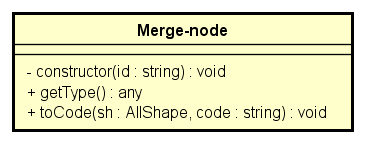
\includegraphics[scale=0.8]{res/sections/SpecificaFrontEnd/Services/Disegnetti/merge-node.png}
	\caption{Diagramma della classe Merge-node}
\end{figure}

\begin{itemize}
	\item \textbf{Descrizione:}\\
	
	\item \textbf{Utilizzo:}\\
	
	\item \textbf{Metodi:}
		\begin{itemize}
			\item \emph{-constructor(id: string)}\\
    		\\
    		\textbf{Parametri:}
    		\begin{itemize}
    			\item \emph{id: string}\\
    			
    		\end{itemize}
    		\item \emph{+getType()}\\
    		
    		\item \emph{+toCode(sh: AllShape, code: string)}\\
    		\\
    		\textbf{Parametri:}
    		\begin{itemize}
    			\item \emph{sh: AllShape}\\
    			
    			\item \emph{code: string}\\
    			
    		\end{itemize}
    	\end{itemize}
\end{itemize}
				
			\paragraph{SWEDesigner::Client::Components::Editor-container::Editor::Metodo}
				\begin{figure}[h!]
	\centering
	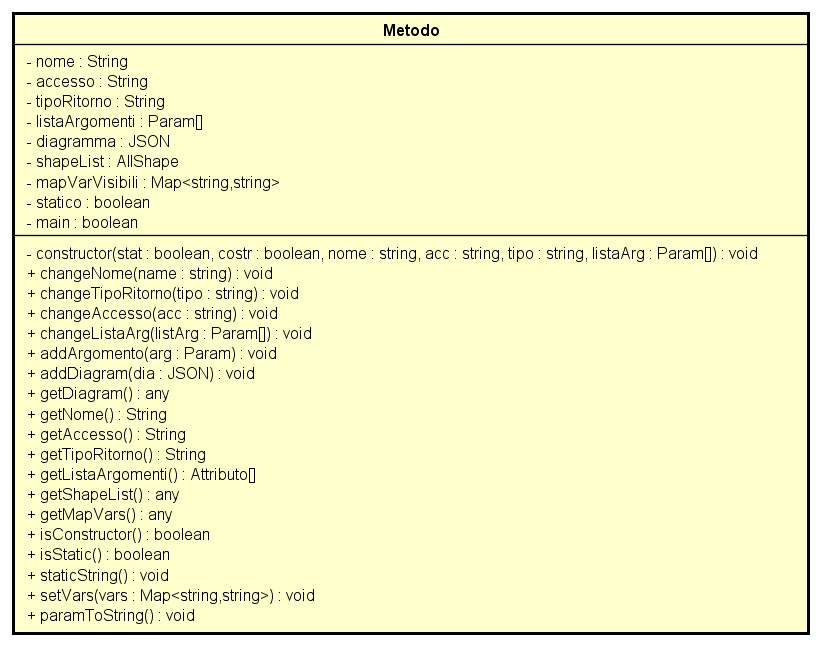
\includegraphics[scale=0.8]{res/sections/SpecificaFrontEnd/Services/Disegnetti/metodo.png}
	\caption{Diagramma della classe Metodo}
\end{figure}

\begin{itemize}
	\item \textbf{Descrizione:}\\
	
	\item \textbf{Utilizzo:}\\
	
	\item \textbf{Metodi:}
		\begin{itemize}
			\item \emph{-nome: string}\\
    		Nome del metodo
    		\item \emph{-accesso: string}\\
    		Visibilità del metodo
    		\item \emph{-tipoRitorno: string}\\
    		Tipo di ritorno del metodo
    		\item \emph{-listaArgomenti: Param[]}\\
    		Lista di argomenti del metodo
    		\item \emph{-diagramma: JSON}\\
    		Definisce il metodo corrente in formato JSON
    		\item \emph{-shapeList: AllShape}\\
    		Lista delle shapes
    		\item \emph{-statico: boolean}\\
    		True se il metodo è marcato static
    		\item \emph{-main: boolean}\\
    		True se il metodo è main
		\end{itemize}
	\item \textbf{Metodi:}
		\begin{itemize}
			\item \emph{-constructor(stat: boolean, costr: boolean, nome: string, acc: string, tipo: string, listaArg: Param[])}\\
    		Costruisce il metodo\\
    		\textbf{Parametri:}
    		\begin{itemize}
    			\item \emph{stat: boolean}\\
    			True se il metodo deve essere marcato static
    			\item \emph{costr: boolean}\\
    			True se il metodo è un costruttore
    			\item \emph{nome: string}\\
    			Nome del metodo da creare
    			\item \emph{acc: string}\\
    			Visibilità del metodo
    			\item \emph{tipo: string}\\
    			Tipo di ritorno del metodo
    			\item \emph{listaArg: Param[]}\\
    			Lista degli argomenti del metodo
    		\end{itemize}
    		\item \emph{+changeNome(name: string)}\\
    		Modifica il nome del metodo selezionato\\
    		\textbf{Parametri:}
    		\begin{itemize}
    			\item \emph{name: string}\\
    			Nuovo nome del metodo
    		\end{itemize}
    		\item \emph{+changeTipoRitorno(tipo: string)}\\
    		Modifica il tipo di ritorno del metodo\\
    		\textbf{Parametri:}
    		\begin{itemize}
    			\item \emph{tipo: string}\\
    			Tipo di ritorno
    		\end{itemize}
    		\item \emph{+changeAccesso(acc: string)}\\
    		Modifica la visibilità del metodo\\
    		\textbf{Parametri:}
    		\begin{itemize}
    			\item \emph{acc: string}\\
    			Visibilità del metodo
    		\end{itemize}
    		\item \emph{+changeListaArg(listArg: Param[])}\\
    		Modifica la lista degli argomenti del metodo\\
    		\textbf{Parametri:}
    		\begin{itemize}
    			\item \emph{listArg: Param[]}\\
    			Lista degli argomenti
    		\end{itemize}
    		\item \emph{+addArgomento(arg: Param)}\\
    		Aggiunge un argomento al metodo\\
    		\textbf{Parametri:}
    		\begin{itemize}
    			\item \emph{arg: Param}\\
    			Argomento da aggiungere
    		\end{itemize}
    		\item \emph{+addDiagram(dia: JSON)}\\
    		Assegna il file JSON all'attributo diagramma della classe\\
    		\textbf{Parametri:}
    		\begin{itemize}
    			\item \emph{dia: JSON}\\
    			File JSON
    		\end{itemize}
    		\item \emph{+getDiagram()}\\
    		Ritorna l'attributo diagramma
    		\item \emph{+getNome()}\\
    		Ritorna il nome del metodo
    		\item \emph{+getAccesso()}\\
    		Ritorna la visibilità del metodo
    		\item \emph{+getTipoRitorno()}\\
    		Ritorna il tipo di ritorno del metodo
    		\item \emph{+getListaArgomenti()}\\
    		Ritorna la lista degli argomenti del metodo
    		\item \emph{+getShapeList()}\\
    		Ritorna la lista della shape
    		\item \emph{+isConstructor()}\\
    		True se è un contruttore
    		\item \emph{+isStatic()}\\
    		True se è marcato static
    		\item \emph{+staticString()}\\
    		Aggiunge la stringa static al metodo
    		\item \emph{+setVars(vars: Map<string, string>)}\\
    		Setta la dichiarazione delle variabili nel metodo\\
    		\textbf{Parametri:}
    		\begin{itemize}
    			\item \emph{vars: Map<string, string>}\\
    			Variabili
    		\end{itemize}
    		\item \emph{+paramToString()}\\
    		Traduce i parametri dei metodi in string
    	\end{itemize}
\end{itemize}
				
			\paragraph{SWEDesigner::Client::Components::Editor-container::Editor::Operation}
				\begin{figure}[h!]
	\centering
	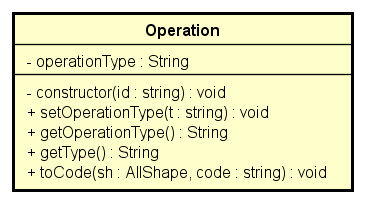
\includegraphics[scale=0.8]{res/sections/SpecificaFrontEnd/Services/Disegnetti/operation.png}
	\caption{Diagramma della classe Operation}
\end{figure}

\begin{itemize}
	\item \textbf{Descrizione:}\\
	
	\item \textbf{Utilizzo:}\\
	
	\item \textbf{Metodi:}
		\begin{itemize}
			\item \emph{-operationType : string}\\
    		
		\end{itemize}
	\item \textbf{Metodi:}
		\begin{itemize}
			\item \emph{-constructor(id: string)}\\
    		\\
    		\textbf{Parametri:}
    		\begin{itemize}
    			\item \emph{id: string}\\
    			
    		\end{itemize}
    		\item \emph{+setOperationType(t: string)}\\
    		\\
    		\textbf{Parametri:}
    		\begin{itemize}
    			\item \emph{t: string}\\
    			
    		\end{itemize}
    		\item \emph{+getOperationType()}\\
    		
    		\item \emph{+getType()}\\
    		
    		\item \emph{+toCode(sh: AllShape, code: string)}\\
    		\\
    		\textbf{Parametri:}
    		\begin{itemize}
    			\item \emph{sh: AllShape}\\
    			
    			\item \emph{code: string}\\
    			
    		\end{itemize}
    	\end{itemize}
\end{itemize}
				
			\paragraph{SWEDesigner::Client::Components::Editor-container::Editor::Operazione}
				\input{res/sections/SpecificaFrontEnd/Services/operazione.tex}
				
			\paragraph{SWEDesigner::Client::Components::Editor-container::Editor::Param}
				\begin{itemize}
	\item \textbf{Descrizione:}\\
	
	\item \textbf{Utilizzo:}\\
	
	\item \textbf{Metodi:}
		\begin{itemize}
			\item \emph{-type: string}\\
    		Tipo del parametro
    		\item \emph{-name: string}\\
    		Nome del parametro
		\end{itemize}
	\item \textbf{Metodi:}
		\begin{itemize}
			\item \emph{-constructor(tipo: string, nome: string)}\\
    		Costruisce un nuovo parametro\\
    		\textbf{Parametri:}
    		\begin{itemize}
    			\item \emph{tipo: string}\\
    			Tipo del parametro
    			\item \emph{nome: string}\\
    			Nome del parametro
    		\end{itemize}
    		\item \emph{+getTipo()}\\
    		Ritorna il tipo del parametro
    		\item \emph{+getNome()}\\
    		Ritorna il nome del parametro
    		\item \emph{+toString()}\\
    		
    		\item \emph{+changeTipo(tipo: string)}\\
    		Modifica il tipo del parametro\\
    		\textbf{Parametri:}
    		\begin{itemize}
    			\item \emph{tipo: string}\\
    			Tipo del parametro
    		\end{itemize}
    		\item \emph{+changeTipo(tipo: string)}\\
    		Modifica il nome del parametro\\
    		\textbf{Parametri:}
    		\begin{itemize}
    			\item \emph{tipo: string}\\
    			Nome del parametro
    		\end{itemize}
    	\end{itemize}
\end{itemize}
				
			\paragraph{SWEDesigner::Client::Components::Editor-container::Editor::Shape}
				\begin{itemize}
	\item \textbf{Descrizione:}\\
	
	\item \textbf{Utilizzo:}\\
	
	\item \textbf{Metodi:}
		\begin{itemize}
			\item \emph{-id: string}\\
    		
    		\item \emph{-succ: string}\\
    		
    		\item \emph{-body: string}\\
    		
    		\item \emph{-printed: boolean}\\
    		
    		\item \emph{-ifPassed: String[]}\\
    		
		\end{itemize}
	\item \textbf{Metodi:}
		\begin{itemize}
			\item \emph{-constructor(id: string)}\\
    		\\
    		\textbf{Parametri:}
    		\begin{itemize}
    			\item \emph{id: string}\\
    			
    		\end{itemize}
    		\item \emph{+setId(id: string)}\\
    		\\
    		\textbf{Parametri:}
    		\begin{itemize}
    			\item \emph{id: string}\\
    			
    		\end{itemize}
    		\item \emph{+setBody(body: string)}\\
    		\\
    		\textbf{Parametri:}
    		\begin{itemize}
    			\item \emph{body: string}\\
    			
    		\end{itemize}
    		\item \emph{+setSucc(succ: string)}\\
    		\\
    		\textbf{Parametri:}
    		\begin{itemize}
    			\item \emph{succ: string}\\
    			
    		\end{itemize}
    		\item \emph{+setIfPassed(pas: string[])}\\
    		\\
    		\textbf{Parametri:}
    		\begin{itemize}
    			\item \emph{pas: string[]}\\
    			
    		\end{itemize}
    		\item \emph{+setPrinted(printed: boolean)}\\
    		\\
    		\textbf{Parametri:}
    		\begin{itemize}
    			\item \emph{printed: boolean}\\
    			
    		\end{itemize}
    		\item \emph{+addBody(b: string)}\\
    		\\
    		\textbf{Parametri:}
    		\begin{itemize}
    			\item \emph{b: string}\\
    			
    		\end{itemize}
    		\item \emph{+getId()}\\
    		
    		\item \emph{+getBody()}\\
    		
    		\item \emph{+getSucc()}\\
    		
    		\item \emph{+getIfPassed()}\\
    		
    		\item \emph{+getPrinted()}\\
    		
    	\end{itemize}
\end{itemize}
				
			\paragraph{SWEDesigner::Client::Components::Editor-container::Editor::Start}
				\begin{figure}[h!]
	\centering
	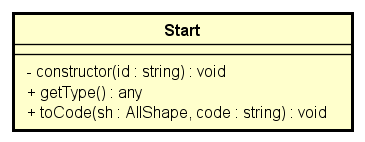
\includegraphics[scale=0.8]{res/sections/SpecificaFrontEnd/Services/Disegnetti/start.png}
	\caption{Diagramma della classe Start}
\end{figure}

\begin{itemize}
	\item \textbf{Descrizione:}\\
	Gestisce la shape stat del diagramma delle attività.
	\item \textbf{Utilizzo:}\\
	Viene utilizzato dal component padre per la gestione del diagramma delle attività.
	\item \textbf{Metodi:}
		\begin{itemize}
			\item \emph{-constructor(id : string)}\\
    		Costruttore della classe\\
    		\textbf{Parametri:}
    		\begin{itemize}
    			\item \emph{id : string}\\
    			Id della shape
    		\end{itemize}
    		\item \emph{+getType()}\\
    		Ritorna il tipo della shape
    		\item \emph{+toCode(sh: AllShape, code: string)}\\
    		Traduce la shape in codice\\
    		\textbf{Parametri:}
    		\begin{itemize}
    			\item \emph{sh: AllShape}\\
    			Shape da tradurre
    			\item \emph{code: string}\\
    			Stringa di codice
    		\end{itemize}
    	\end{itemize}
\end{itemize}
				
			\paragraph{SWEDesigner::Client::Components::Editor-container::Editor::Variabile}
				\begin{itemize}
	\item \textbf{Descrizione:}\\
	
	\item \textbf{Utilizzo:}\\
	
	\item \textbf{Metodi:}
		\begin{itemize}
			\item \emph{-type: string}\\
    		
    		\item \emph{-name: string}\\
    		
    		\item \emph{-value: string}\\
    		
		\end{itemize}
	\item \textbf{Metodi:}
		\begin{itemize}
			\item \emph{-constructor(type: string, name: string, value: string)}\\
    		\\
    		\textbf{Parametri:}
    		\begin{itemize}
    			\item \emph{type: string}\\
    			
    			\item \emph{name: string}\\
    			
    			\item \emph{value: string}\\
    			
    		\end{itemize}
    		\item \emph{+getType()}\\
    		
    		\item \emph{+getName()}\\
    		
    		\item \emph{+getValue()}\\
    		
    		\item \emph{+setType(type: string)}\\
    		\\
    		\textbf{Parametri:}
    		\begin{itemize}
    			\item \emph{type: string}\\
    			
    		\end{itemize}
    		\item \emph{+setName(name: string)}\\
    		\\
    		\textbf{Parametri:}
    		\begin{itemize}
    			\item \emph{name: string}\\
    			
    		\end{itemize}
    		\item \emph{+setValue(value: string)}\\
    		\\
    		\textbf{Parametri:}
    		\begin{itemize}
    			\item \emph{value: string}\\
    			
    		\end{itemize}
    	\end{itemize}
\end{itemize}
				
			\paragraph{SWEDesigner::Client::Components::Editor-container::Editor::While-node}
				\begin{figure}[h!]
	\centering
	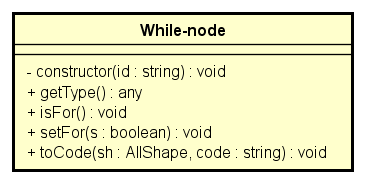
\includegraphics[scale=0.8]{res/sections/SpecificaFrontEnd/Services/Disegnetti/while-node.png}
	\caption{Diagramma della classe While-node}
\end{figure}

\begin{itemize}
	\item \textbf{Descrizione:}\\
	
	\item \textbf{Utilizzo:}\\
	
	\item \textbf{Metodi:}
		\begin{itemize}
			\item \emph{-constructor(id: string)}\\
    		Costruttore della classe\\
    		\textbf{Parametri:}
    		\begin{itemize}
    			\item \emph{id: string}\\
    			Id della shape
    		\end{itemize}
    		\item \emph{+getType()}\\
    		Ritorna il tipo della shape
    		\item \emph{+isFor()}\\
    		Ritorna il valore del for
    		\item \emph{+setFor(s: boolean)}\\
    		Setta il for\\
    		\textbf{Parametri:}
    		\begin{itemize}
    			\item \emph{s: boolean}\\
    			Valore del for
    		\end{itemize}
    		\item \emph{+toCode(sh: AllShape, code: string)}\\
    		Traduce la shape in codice\\
    		\textbf{Parametri:}
    		\begin{itemize}
    			\item \emph{sh: AllShape}\\
    			Shape da tradurre
    			\item \emph{code: string}\\
    			Stringa di codice
    		\end{itemize}
    	\end{itemize}
\end{itemize}
				
	\subsection{SWEDesigner::Client::Components::Editor-container::Editor::Edit-class-menu}
		\subsubsection{Informazioni generali}
			\begin{itemize}
          		\item \textbf{Descrizione:}\\
          		
          		\item \textbf{Padre:} SWEDesigner::Client::Components::Editor-container::Editor
          	\end{itemize}

         \subsubsection{Classi}
         
         	\paragraph{SWEDesigner::Client::Components::Editor-container::Editor::Edit-class-menu::Edit-class-menuComponent}
				\input{res/sections/SpecificaFrontEnd/Components/edit-class-menu.tex}
				
			\paragraph{SWEDesigner::Client::Components::Editor-container::Editor::Edit-class-menu::Change-class-nameComponent}
				\begin{figure}[h!]
	\centering
	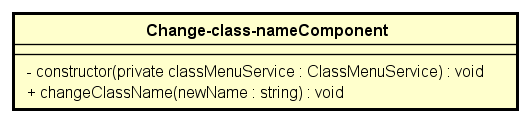
\includegraphics[scale=0.8]{res/sections/SpecificaFrontEnd/Components/Disegnetti/change-class-name.png}
	\caption{Diagramma della classe Change-class-name}
\end{figure}

\begin{itemize}
	\item \textbf{Descrizione:}\\
	Gestisce il cambiamento del nome della shape selezionata.
	\item \textbf{Utilizzo:}\\
	Viene utilizzata da EditClassMenuComponent per gestire la rinominazione delle shapes.
	\item \textbf{Metodi:}
		\begin{itemize}
			\item \emph{-constructor(private classMenuService: ClassMenuService)}\\
    		Costruttore della classe\\
    		\textbf{Parametri:}
    		\begin{itemize}
    			\item \emph{classMenuService: ClassMenuService}\\
    			Serve per creare un istanziazione di ClassMenuService
    		\end{itemize}
    		\item \emph{+changeClassName(newName: string)}\\
    		Modifica il nome della classe\\
    		\textbf{Parametri:}
    		\begin{itemize}
    			\item \emph{newName: string}\\
    			Nome della classe
    		\end{itemize}
		\end{itemize}
\end{itemize}
				
			\paragraph{SWEDesigner::Client::Components::Editor-container::Editor::Edit-class-menu::Class-add-attributeComponent}
				\begin{figure}[h!]
	\centering
	\includegraphics[scale=0.8]{res/sections/SpecificaFrontEnd/Components/Disegnetti/class-add-atribute.png}
	\caption{Diagramma della classe Class-add-attribute}
\end{figure}

\begin{itemize}
	\item \textbf{Descrizione:}\\
	
	\item \textbf{Utilizzo:}\\
	
	\item \textbf{Metodi:}
		\begin{itemize}
			\item \emph{-constructor(private classMenuService: ClassMenuService)}\\
    		Costruttore della classe\\
    		\textbf{Parametri:}
    		\begin{itemize}
    			\item \emph{classMenuService: ClassMenuService}\\
    			Serve per creare un istanziazione di ClassMenuService
    		\end{itemize}
    		\item \emph{+justOneCheckbox(event: any)}\\
    		Controlla che ci sia solo un elemento sulla checkbox attributo\\
    		\textbf{Parametri:}
    		\begin{itemize}
    			\item \emph{event: any}\\
    			Nome dell'elemento
    		\end{itemize}
    		\item \emph{+addAttributo(nome: string, staticAtt: boolean, finalAtt: boolean, tipo: string, acc: string) }\\
    		Aggiunge un nuovo attributo\\
    		\textbf{Parametri:}
    		\begin{itemize}
    			\item \emph{nome: string}\\
    			Nome dell'attributo
    			\item \emph{staticAtt: boolean}\\
    			True se è marcato static
    			\item \emph{finalAtt: boolean}\\
    			True se è marcato final
    			\item \emph{tipo: string}\\
    			Tipo dell'attributo
    			\item \emph{acc: string}\\
    			Visibilità dell'attributo
    		\end{itemize}
		\end{itemize}
\end{itemize}
				
			\paragraph{SWEDesigner::Client::Components::Editor-container::Editor::Edit-class-menu::Class-add-main-methodComponent}
				\begin{itemize}
	\item \textbf{Descrizione:}\\
	
	\item \textbf{Utilizzo:}\\
	
	\item \textbf{Metodi:}
		\begin{itemize}
			\item \emph{-constructor(private classMenuService: ClassMenuService)}\\
    		Costruttore della classe\\
    		\textbf{Parametri:}
    		\begin{itemize}
    			\item \emph{classMenuService: ClassMenuService}\\
    			Crea un istanziazione di ClassMenuService
    		\end{itemize}
    		\item \emph{addMain()}\\
    		Aggiunge il metodo main alla classe selezionata
		\end{itemize}
\end{itemize}
				
			\paragraph{SWEDesigner::Client::Components::Editor-container::Editor::Edit-class-menu::Class-add-methodComponent}
				\begin{itemize}
	\item \textbf{Descrizione:}\\
	
	\item \textbf{Utilizzo:}\\
	
	\item \textbf{Metodi:}
		\begin{itemize}
			\item \emph{-constructor(private classMenuService: ClassMenuService)}\\
    		Costruttore della classe\\
    		\textbf{Parametri:}
    		\begin{itemize}
    			\item \emph{classMenuService: ClassMenuService}\\
    			Crea un istanziazione di ClassMenuService
    		\end{itemize}
    		\item \emph{+addParam(type: string, name: string)}\\
    		Aggiunge un parametro alla lista dei parametri del metodo\\
    		\textbf{Parametri:}
    		\begin{itemize}
    			\item \emph{type: string}\\
    			Tipo del parametro
    			\item \emph{name: string}\\
    			Nome del parametro
    		\end{itemize}
    		\item \emph{+removeParam(type: string, name: string)}\\
    		Rimuove un parametro dalla lista dei parametri del metodo\\
    		\textbf{Parametri:}
    		\begin{itemize}
    			\item \emph{type: string}\\
    			Tipo del parametro
    			\item \emph{name: string}\\
    			Nome del parametro
    		\end{itemize}
    		\item \emph{+addMetodo(nome: string, staticMet: boolean, constructor: boolean, tipo: string, acc: string)}\\
    		Aggiunge un nuovo metodo\\
    		\textbf{Parametri:}
    		\begin{itemize}
    			\item \emph{nome: string}\\
    			Nome del metodo
    			\item \emph{staticMet: boolean}\\
    			True se è marcato static
    			\item \emph{constructor: boolean}\\
    			True se è un costruttore
    			\item \emph{tipo: string}\\
    			Tipo di ritorno del metodo
    			\item \emph{acc: string}\\
    			Visibilità del metodo
    		\end{itemize}
    		\item \emph{+justOneCheckbox(event: any)}\\
    		Controlla che ci sia solo un elemento sulla checkbox\\
    		\textbf{Parametri:}
    		\begin{itemize}
    			\item \emph{event: any}\\
    			Nome dell'elemento
    		\end{itemize}
		\end{itemize}
\end{itemize}
				
			\paragraph{SWEDesigner::Client::Components::Editor-container::Editor::Edit-class-menu::Class-list-attributeComponent}
				\begin{itemize}
	\item \textbf{Descrizione:}\\
	
	\item \textbf{Utilizzo:}\\
	
	\item \textbf{Metodi:}
		\begin{itemize}
			\item \emph{-constructor(private classMenuService: ClassMenuService)}\\
    		Costruttore della classe\\
    		\textbf{Parametri:}
    		\begin{itemize}
    			\item \emph{classMenuService: ClassMenuService}\\
    			Crea un istanziazione di ClassMenuService
    		\end{itemize}
    		\item \emph{+changeAttributo(newName: string, oldName: string, tipo: string, acc: string, stat: boolean, final: boolean)}\\
    		Modifica le proprietà di un attributo\\
    		\textbf{Parametri:}
    		\begin{itemize}
    			\item \emph{newName: string}\\
    			Nuovo nome dell'attributo
    			\item \emph{oldName: string}\\
    			Vecchio nome dell'attributo
    			\item \emph{tipo: string}\\
    			Tipo dell'attributo
    			\item \emph{acc: string}\\
    			Visibilità dell'attributo
    			\item \emph{stat: boolean}\\
    			True se è marcato static
    			\item \emph{final: boolean}\\
    			True se è marcato final
    		\end{itemize}
    		\item \emph{+justOneCheckbox(event: any)}\\
    		Controlla che ci sia solo un elemento sulla checkbox\\
    		\textbf{Parametri:}
    		\begin{itemize}
    			\item \emph{event: any}\\
    			Nome dell'elemento
    		\end{itemize}
		\end{itemize}
\end{itemize}
				
			\paragraph{SWEDesigner::Client::Components::Editor-container::Editor::Edit-class-menu::Class-list-methodComponent}
				\begin{figure}[h!]
	\centering
	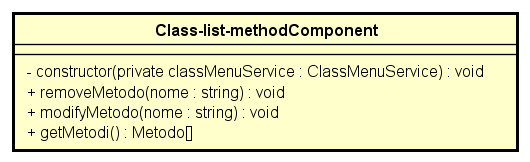
\includegraphics[scale=0.8]{res/sections/SpecificaFrontEnd/Components/Disegnetti/class-list-method.png}
	\caption{Diagramma della classe Class-list-method}
\end{figure}

\begin{itemize}
	\item \textbf{Descrizione:}\\
	Serve a mostrare la lista dei metodi di una classe.
	\item \textbf{Utilizzo:}\\
	Viene utilizzato da EditClassMenuComponent per visualizzare la lista dei metodi delle classi.
	\item \textbf{Metodi:}
		\begin{itemize}
			\item \emph{-constructor(private classMenuService: ClassMenuService)}\\
    		Costruttore della classe\\
    		\textbf{Parametri:}
    		\begin{itemize}
    			\item \emph{classMenuService: ClassMenuService}\\
    			Crea un istanziazione di ClassMenuService
    		\end{itemize}
    		\item \emph{+removeMetodo(nome: string)}\\
    		Rimuove un metodo\\
    		\textbf{Parametri:}
    		\begin{itemize}
    			\item \emph{nome: string}\\
    			Nome del metodo da rimuovere
    		\end{itemize}
    		\item \emph{+modifyMetodo(nome: string)}\\
    		Modifica il corpo del metodo\\
    		\textbf{Parametri:}
    		\begin{itemize}
    			\item \emph{nome: string}\\
    			Nome del metodo
    		\end{itemize}
    		\item \emph{+getMetodi()}\\
    		Ritorna la lista dei metodi
		\end{itemize}
\end{itemize}
				
			\paragraph{SWEDesigner::Client::Components::Editor-container::Editor::Edit-class-menu::Display-class-nameComponent}
				\begin{figure}[h!]
	\centering
	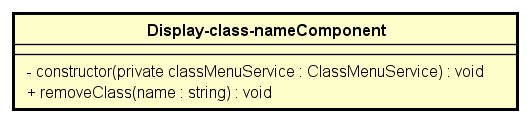
\includegraphics[scale=0.8]{res/sections/SpecificaFrontEnd/Components/Disegnetti/display-class-name.png}
	\caption{Diagramma della classe Display-class-name}
\end{figure}

\begin{itemize}
	\item \textbf{Descrizione:}\\
	Serve per mostrare il nome della classe.
	\item \textbf{Utilizzo:}\\
	Viene utilizata da EditClassMenuComponent per visualizzare i nomi delle classi.
	\item \textbf{Metodi:}
		\begin{itemize}
			\item \emph{-constructor(private classMenuService: ClassMenuService)}\\
    		Costruttore della classe\\
    		\textbf{Parametri:}
    		\begin{itemize}
    			\item \emph{classMenuService: ClassMenuService}\\
    			Crea un istanziazione di ClassMenuService
    		\end{itemize}
    		\item \emph{+removeClass(name: string)}\\
    		Rimuove la classe selezionata\\
    		\textbf{Parametri:}
    		\begin{itemize}
    			\item \emph{name: string}\\
    			Nome della classe da eliminare
    		\end{itemize}
		\end{itemize}
\end{itemize}
		
	\subsection{SWEDesigner::Client::Services}
		\subsubsection{Informazioni generali}
			\begin{itemize}
          		\item \textbf{Descrizione:}\\
          		Il package contiene i servizi per le operazioni di iterazione tra i component e il server.
          		\item \textbf{Padre:} SWEDesigner::Client
          		\item \textbf{Package contenuti:}\\
          		\begin{itemize}
          			\item Models\\
          			Il package contiene moduli necessari a storicizzare i dati inseriti all’interno dei diagrammi.
          		\end{itemize}
          	\end{itemize}
          	
          \subsubsection{Classi}
          
          	\paragraph{SWEDesigner::Client::Services::AccountService}
				\begin{figure}[h!]
	\centering
	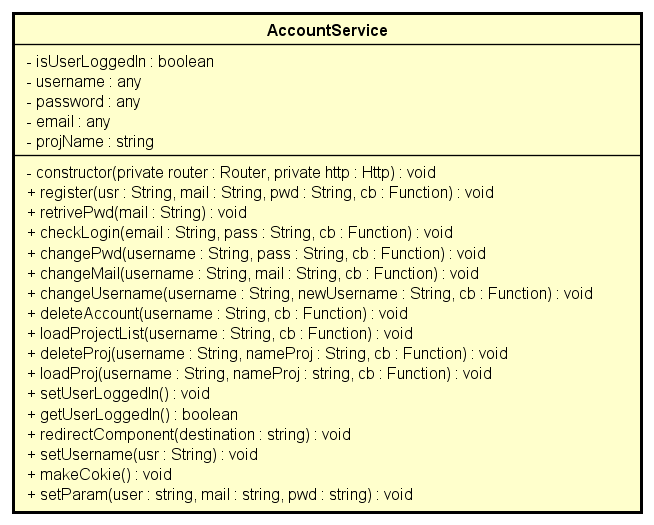
\includegraphics[scale=0.8]{res/sections/SpecificaFrontEnd/Services/Disegnetti/account.png}
	\caption{Diagramma della classe AccountService}
\end{figure}

\begin{itemize}
	\item \textbf{Descrizione:}\\
	
	\item \textbf{Utilizzo:}\\
	
	\item \textbf{Attributi:}
		\begin{itemize}
			\item \emph{-isUserLoggedIn: boolean}\\
			Serve a controllare se l'utente è autenticato
			\item \emph{-username: any}\\
			Contiene l'username dell'utente
			\item \emph{-password: any}\\
			Contiene la password dell'utente
			\item \emph{-email: any}\\
			Contiene l'email dell'utente
			\item \emph{-notOpenedProj: boolean}\\
			Controlla se il progetto è aperto o meno
			\item \emph{-projName: string}\\
			Contiene il nome del progetto attualmente aperto
		\end{itemize}
	\item \textbf{Metodi:}
		\begin{itemize}
			\item \emph{-constructor(private router: Router,private http: Http)}\\
    		Costruttore della classe\\
    		\textbf{Parametri:}
    		\begin{itemize}
    			\item \emph{router: Router}\\
    			Crea una nuova istanziazione di Router
    			\item \emph{http: Http}\\
    			Crea una nuova istanziazione di Http
    		\end{itemize}
    		\item \emph{+register(usr: String, mail: String, pwd: String, cb: Function)}\\
    		Serve per registrare un nuovo utente\\
    		\textbf{Parametri:}
    		\begin{itemize}
    			\item \emph{usr: String}\\
    			Nome utente
    			\item \emph{mail: String}\\
    			Email dell'utente
    			\item \emph{pwd: String}\\
    			Password dell'utente
    			\item \emph{cb: Function}\\
    			
    		\end{itemize}
    		\item \emph{+retrivePwd(mail: String)}\\
    		Serve per recuperare la password di un utente\\
    		\textbf{Parametri:}
    		\begin{itemize}
    			\item \emph{mail: String}\\
    			Email a cui mandare la password
    		\end{itemize}
    		\item \emph{+checkLogin(email: String, pass: String, cb: Function)}\\
    		Serve per effettuare l'autenticazione di un utente\\
    		\textbf{Parametri:}
    		\begin{itemize}
    			\item \emph{email: String}\\
    			Email dell'utente
    			\item \emph{pass: String}\\
    			Password dell'utente
    			\item \emph{cb: Function}\\
    			
    		\end{itemize}
    		\item \emph{+changePwd(username: String, pass: String, cb: Function)}\\
    		Serve per modificare la password di un utente\\
    		\textbf{Parametri:}
    		\begin{itemize}
    			\item \emph{username: String}\\
    			Nome utente
    			\item \emph{pass: String}\\
    			Password dell'utente
    			\item \emph{cb: Function}\\
    			
    		\end{itemize}
    		\item \emph{+changeMail(username: String, mail: String, cb:Function)}\\
    		Serve per modificare la mail dell'utente\\
    		\textbf{Parametri:}
    		\begin{itemize}
    			\item \emph{username: String}\\
    			Nome utente
    			\item \emph{mail: String}\\
    			Email dell'utente
    			\item \emph{String, cb:Function}\\
    			
    		\end{itemize}
    		\item \emph{+changeUsername(username: String, newUsername: String, cb: Function)}\\
    		Serve per modificare l'username dell'utente\\
    		\textbf{Parametri:}
    		\begin{itemize}
    			\item \emph{username: String}\\
    			Nome utente
    			\item \emph{newUsername: String}\\
    			Nuovo username
    			\item \emph{cb: Function}\\
    			
    		\end{itemize}
    		\item \emph{+deleteAccount(username: String, cb: Function)}\\
    		Serve per eliminare un account\\
    		\textbf{Parametri:}
    		\begin{itemize}
    			\item \emph{username: String}\\
    			Nome utente
    			\item \emph{cb: Function}\\
    			
    		\end{itemize}
    		\item \emph{+loadProjectList(username: String, cb: Function)}\\
    		Serve a caricare la lista dei progetti\\
    		\textbf{Parametri:}
    		\begin{itemize}
    			\item \emph{username: String}\\
    			Nome utente
    			\item \emph{cb: Function}\\
    			
    		\end{itemize}
    		\item \emph{+deleteProj(username: String, nameProj: String, cb: Function)}\\
    		Serve per eliminare un progetto\\
    		\textbf{Parametri:}
    		\begin{itemize}
    			\item \emph{username: String}\\
    			Nome utente
    			\item \emph{nameProj: String}\\
    			Nome del progetto
    			\item \emph{cb: Function}\\
    			
    		\end{itemize}
    		\item \emph{+loadProj(username: String, nameProj: string, cb: Function)}\\
    		Carica un progetto dalla lista progetti dell'utente\\
    		\textbf{Parametri:}
    		\begin{itemize}
    			\item \emph{username: String}\\
    			Nome utente
    			\item \emph{nameProj: string}\\
    			Nome del progetto
    			\item \emph{cb: Function}\\
    			
    		\end{itemize}
    		\item \emph{+setUserLoggedIn()}\\
    		Modifica lo stato di autenticazione dell'utente
    		\item \emph{+getUserLoggedIn()}\\
    		Ritorna true se l'utente è autenticato
    		\item \emph{+redirectComponent(destination:string)}\\
    		Questa funzione reindirizza questo componente al componente destinazione\\
    		\textbf{Parametri:}
    		\begin{itemize}
    			\item \emph{destination:string}\\
    			Componente destinazione
    		\end{itemize}
    		\item \emph{+setUsername(usr: String)}\\
    		Setta l'username dell'utente\\
    		\textbf{Parametri:}
    		\begin{itemize}
    			\item \emph{usr: String}\\
    			Nome utente
    		\end{itemize}
    		\item \emph{+makeCokie()}\\
    		Costruisce dei cookie di sessione contenenti le informazioni dell'utente
    		\item \emph{+setParam(user: string, mail:string, pwd: string)}\\
    		Setta le informazione in AccountService\\
    		\textbf{Parametri:}
    		\begin{itemize}
    			\item \emph{user: string}\\
    			Nome utente
    			\item \emph{mail:string}\\
    			Email dell'utente
    			\item \emph{pwd: string}\\
    			Password dell'utente
    		\end{itemize}
    		\item \emph{+logout()}\\
    		Esegue il logout
		\end{itemize}
\end{itemize}
				
			\paragraph{SWEDesigner::Client::Services::Main-editorService}
				\begin{figure}[h!]
	\centering
	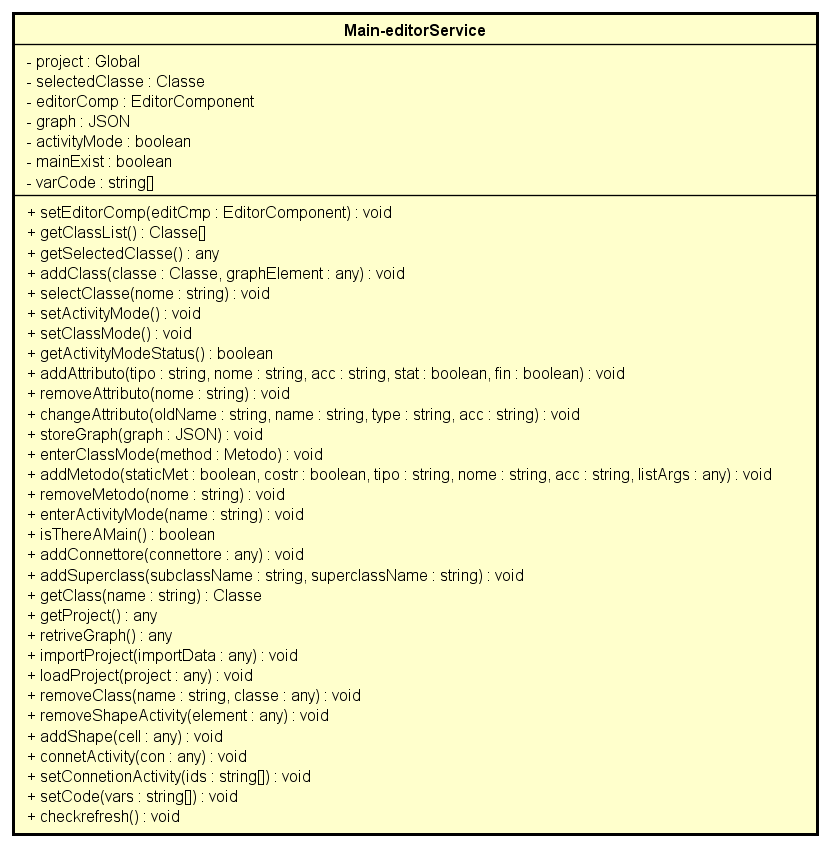
\includegraphics[scale=0.8]{res/sections/SpecificaFrontEnd/Services/Disegnetti/main-editor.png}
	\caption{Diagramma della classe Main-editorService}
\end{figure}

\begin{itemize}
	\item \textbf{Descrizione:}\\
	
	\item \textbf{Utilizzo:}\\
	
	\item \textbf{Attributi:}
		\begin{itemize}
			\item \emph{-project: Global}\\
			Serve per memorizzare informazioni riguardo il progetto corrente
			\item \emph{-selectedClasse: Classe}\\
			Memorizza la classe corrispondente nel canvas dell'editor
			\item \emph{-editorComp: EditorComponent}\\
			Serve per accedere direttamente all'EditorComponent
			\item \emph{-graph: JSON}\\
			Serve per memorizzare il grafico dell'editor
			\item \emph{-activityMode: boolean}\\
			Indica se è in uso l'activity diagram
			\item \emph{-mainExist: boolean}\\
			Indica se esiste il metodo main
			\item \emph{-varCode: string[]}\\
			
		\end{itemize}
	\item \textbf{Metodi:}
		\begin{itemize}
			\item \emph{+setEditorComp(editCmp: EditorComponent)}\\
    		Serve per costruire un istanziazione dell'EditorComponent\\
    		\textbf{Parametri:}
    		\begin{itemize}
    			\item \emph{editCmp: EditorComponent}\\
    			Istanzia EditorComponent
    		\end{itemize}
    		\item \emph{+getClassList()}\\
    		Ritorna la lista delle classi presenti nel progetto
    		\item \emph{+getSelectedClasse()}\\
    		Ritorna la classe selezionata
    		\item \emph{+addClass(classe: Classe, graphElement: any)}\\
    		Aggiunge un oggetto di tipo classe\\
    		\textbf{Parametri:}
    		\begin{itemize}
    			\item \emph{classe: Classe}\\
    			Classe da aggiungere
    			\item \emph{graphElement: any}\\
    			Elemento della libreria grafica
    		\end{itemize}
    		\item \emph{+selectClasse(nome: string)}\\
    		Cerca una classe all'interno della lista\\
    		\textbf{Parametri:}
    		\begin{itemize}
    			\item \emph{nome: string}\\
    			Nome della classe da cercare
    		\end{itemize}
    		\item \emph{+setActivityMode()}\\
    		Passa alla modalità activity diagram
    		\item \emph{+setClassMode()}\\
    		Passa alla modalità class diagram
    		\item \emph{+getActivityModeStatus()}\\
    		Ritorna il valore del fral activityMode
    		\item \emph{+addAttributo(tipo: string, nome:string, acc: string, stat: boolean, fin: boolean)}\\
    		Aggiunge un metodo alla selectedClasse\\
    		\textbf{Parametri:}
    		\begin{itemize}
    			\item \emph{tipo: string}\\
    			Tipo dell'attributo
    			\item \emph{nome:string}\\
    			Nome dell'attributo
    			\item \emph{acc: string}\\
    			Visibilità dell'attributo
    			\item \emph{stat: boolean}\\
    			True se è marcato static
    			\item \emph{fin: boolean}\\
    			True se è marcato final
    		\end{itemize}
    		\item \emph{+removeAttributo(nome: string)}\\
    		Rimuove un attributo dalla selectedClasse\\
    		\textbf{Parametri:}
    		\begin{itemize}
    			\item \emph{nome: string}\\
    			Nome dell'attributo da rimuovere
    		\end{itemize}
    		\item \emph{+changeAttributo(oldName: string, name: string, type: string, acc: string)}\\
    		Modifica un attributo della selectedClasse\\
    		\textbf{Parametri:}
    		\begin{itemize}
    			\item \emph{oldName: string}\\
    			Vecchio nome
    			\item \emph{name: string}\\
    			Nuovo nome
    			\item \emph{type: string}\\
    			Tipo dell'attributo
    			\item \emph{acc: string}\\
    			Visibilità dell'attributo
    		\end{itemize}
    		\item \emph{+storeGraph(graph: JSON)}\\
    		Memorizza il grafico\\
    		\textbf{Parametri:}
    		\begin{itemize}
    			\item \emph{graph: JSON}\\
    			Grafico da memorizzare
    		\end{itemize}
    		\item \emph{+enterClassMode(method: Metodo)}\\
    		Serve per ripristinare il diagramma delle classi dopo aver definito un metodo\\
    		\textbf{Parametri:}
    		\begin{itemize}
    			\item \emph{method: Metodo}\\
    			Metodo definito
    		\end{itemize}
    		\item \emph{+addMetodo(staticMet: boolean, costr: boolean, tipo: string, nome:string, acc: string, listArgs: any)}\\
    		Aggiunge un nuovo metodo alla selectedClasse\\
    		\textbf{Parametri:}
    		\begin{itemize}
    			\item \emph{staticMet: boolean}\\
    			True se è marcato static
    			\item \emph{costr: boolean}\\
    			True se è un costruttore
    			\item \emph{tipo: string}\\
    			Tipo di ritorno del metodo
    			\item \emph{nome:string}\\
    			Nome del metodo
    			\item \emph{acc: string}\\
    			Visibilità del metodo
    			\item \emph{listArgs: any}\\
    			Lista degli argomenti del metodo
    		\end{itemize}
    		\item \emph{+removeMetodo(nome: string)}\\
    		Rimuove un metodo dalla selectedClasse\\
    		\textbf{Parametri:}
    		\begin{itemize}
    			\item \emph{nome: string}\\
    			Nome del metodo da eliminare
    		\end{itemize}
    		\item \emph{+enterActivityMode(name: string)}\\
    		Entra nella modalità activity per modificare il corpo un metodo\\
    		\textbf{Parametri:}
    		\begin{itemize}
    			\item \emph{name: string}\\
    			Nome del metodo da modificare
    		\end{itemize}
    		\item \emph{+isThereAMain()}\\
    		Ritorna true se è presente il metodo main nella selectedClasse
    		\item \emph{+addConnettore(connettore: any)}\\
    		Aggiunge un connettore alla selectedClasse\\
    		\textbf{Parametri:}
    		\begin{itemize}
    			\item \emph{connettore: any}\\
    			Conettore da aggiungere
    		\end{itemize}
    		\item \emph{+addSuperclass(subclassName: string, superclassName: string)}\\
    		\\
    		\textbf{Parametri:}
    		\begin{itemize}
    			\item \emph{subclassName: string}\\
    			
    			\item \emph{superclassName: string}\\
    			
    		\end{itemize}
    		\item \emph{+getClass(name: string)}\\
    		\\
    		\textbf{Parametri:}
    		\begin{itemize}
    			\item \emph{name: string}\\
    			
    		\end{itemize}
    		\item \emph{+getProject()}\\
    		
    		\item \emph{+retriveGraph()}\\
    		
    		\item \emph{+importProject(importData: any)}\\
    		\\
    		\textbf{Parametri:}
    		\begin{itemize}
    			\item \emph{importData: any}\\
    			
    		\end{itemize}
    		\item \emph{+loadProject(project: any)}\\
    		\\
    		\textbf{Parametri:}
    		\begin{itemize}
    			\item \emph{project: any}\\
    			
    		\end{itemize}
    		\item \emph{+removeClass(name: string, classe: any)}\\
    		\\
    		\textbf{Parametri:}
    		\begin{itemize}
    			\item \emph{name: string}\\
    			
    			\item \emph{classe: any}\\
    			
    		\end{itemize}
    		\item \emph{+removeShapeActivity(element: any)}\\
    		\\
    		\textbf{Parametri:}
    		\begin{itemize}
    			\item \emph{element: any}\\
    			
    		\end{itemize}
    		\item \emph{addShape(cell: any)}\\
    		\\
    		\textbf{Parametri:}
    		\begin{itemize}
    			\item \emph{cell: any}\\
    			
    		\end{itemize}
    		\item \emph{+connetActivity(con: any)}\\
    		\\
    		\textbf{Parametri:}
    		\begin{itemize}
    			\item \emph{con: any}\\
    			
    		\end{itemize}
    		\item \emph{+setConnetionActivity(ids: string[])}\\
    		\\
    		\textbf{Parametri:}
    		\begin{itemize}
    			\item \emph{ids: string[]}\\
    			
    		\end{itemize}
    		\item \emph{+setCode(vars: string[])}\\
    		\\
    		\textbf{Parametri:}
    		\begin{itemize}
    			\item \emph{vars: string[]}\\
    			
    		\end{itemize}
    		\item \emph{+checkrefresh()}\\
    		
		\end{itemize}
\end{itemize}
				
			\paragraph{SWEDesigner::Client::Services::MenuService}
				\begin{itemize}
	\item \textbf{Descrizione:}\\
	
	\item \textbf{Utilizzo:}\\
	
	\item \textbf{Attributi:}
		\begin{itemize}
			\item \emph{-selectedGraphService: Subject<any>}\\
			
			\item \emph{-importData: any}\\
			
		\end{itemize}
	\item \textbf{Metodi:}
		\begin{itemize}
			\item \emph{+zoomIn()}\\
    		Esegue lo zoom in avanti
    		\item \emph{+zoomOut()}\\
    		Esegue lo zoom all'indietro
    		\item \emph{+copyElement()}\\
    		Copia l'elemento selezionato
    		\item \emph{+pasteElement()}\\
    		Incolla l'elemento copiato/tagliato
    		\item \emph{+cutElement()}\\
    		Taglia l'elemento selezionato
    		\item \emph{+undo()}\\
    		Annulla l'ultima operazione
    		\item \emph{+redo()}\\
    		Ripristina l'azione annullata
    		\item \emph{+elimina()}\\
    		Elimina l'elemento selezionato
    		\item \emph{+saveData(proj: JSON, cb: Function)}\\
    		Richiede al server dei dati del progetto corrente memorizzati nel database\\
    		\textbf{Parametri:}
    		\begin{itemize}
    			\item \emph{proj: JSON}\\
    			Progetto corrente
    			\item \emph{cb: Function}\\
    			
    		\end{itemize}
    		\item \emph{+updateData(proj: JSON, cb: Function)}\\
    		Aggiorna i dati del progetto corrente nel database\\
    		\textbf{Parametri:}
    		\begin{itemize}
    			\item \emph{proj: JSON}\\
    			Progetto corrente
    			\item \emph{cb: Function}\\
    			
    		\end{itemize}
    		\item \emph{+updateName(usr: string, oldName: string, newName: string, cb: Function)}\\
    		Aggiorna il nome del progetto corrente\\
    		\textbf{Parametri:}
    		\begin{itemize}
    			\item \emph{usr: string}\\
    			Nome utente
    			\item \emph{oldName: string}\\
    			Vecchio nome del progetto
    			\item \emph{newName: string}\\
    			Nuovo nome del progetto
    			\item \emph{cb: Function}\\
    			
    		\end{itemize}
    		\item \emph{+encrypt(proj: JSON)}\\
    		Richiede al server la funzione di criptazione\\
    		\textbf{Parametri:}
    		\begin{itemize}
    			\item \emph{proj: JSON}\\
    			Progetto da criptare
    		\end{itemize}
    		\item \emph{+readFile(file: any, onloadCallBack: any)}\\
    		Legge un file esterno\\
    		\textbf{Parametri:}
    		\begin{itemize}
    			\item \emph{file: any}\\
    			File da caricare
    			\item \emph{onloadCallBack: any}\\
    			
    		\end{itemize}
    		\item \emph{+import(event: any)}\\
    		Importa un file esterno\\
    		\textbf{Parametri:}
    		\begin{itemize}
    			\item \emph{event: any}\\
    			File da importare
    		\end{itemize}
    		\item \emph{+getImportData()}\\
    		
    		\item \emph{+donwload()}\\
    		Richiede al server la funzione di parsing e download
    		\item \emph{+code()}\\
    		Richiama la funziona di download
		\end{itemize}
\end{itemize}